% !TeX root = d1.tex

\documentclass{article}

\usepackage{xcolor}
\usepackage[margin=0.5in]{geometry} 
\usepackage{graphicx}
\title{MindMerge --- Deliverable e 1}
\author{Gabriele Benetti, Gioele Berdardini, Luca Fossa Crescini, Luca Sartore}

\begin{document}
\maketitle


\tableofcontents

\section{SWAT Analysis}
\subsection{Strengths}
\begin{itemize}
    \item \textbf{Operating in an market that is hyped and growing: }
          The Artificial intelligence and LLM (large language models) market is currently on everyone's mouth.
          and is growing fast\dots this would make it easy for our team to find sell the product, and potentially find investors

    \item \textbf{The workplace is getting more and more digital: }
          In the last decades more and more jobs are getting used to using

    \item \textbf{: }
    \item \textbf{: }


\end{itemize}
\subsection{Weaknesses}

\subsection{Opportunities}

\subsection{Threads}

\section{Functional Requirements}
\subsection{Authentication and account management}
\begin{itemize}
    \item An user shall be able to perform a login operation
    \item An authenticated user shall be able to perform a logout operation
    \item An authenticated user shall be able to completely delete its account
\end{itemize}
\subsection{Organization management and fee Requirements}
\begin{itemize}
    \item The owner shall be able to pay a subscription for enabling its Organization
    \item The system shall be able to restrict edit permissions if the subscription is not paid
    \item The system must allow users to create an Organization, and therefore becoming its owner
    \item The owner must be able to add and remove users to his Organization
    \item The system must allow Organizations to assign tasks for their assignees
\end{itemize}
\subsection{Task structure}
\begin{itemize}
    \item Each task should be capable of having multiple subtasks in a tree structure
    \item Each task must have exactly one manager
    \item Each task must have at least one assignee
    \item Each task should have a title
    \item Each task should have a description
    \item Each task should have a priority option
    \item Each task should have a deadline option
    \item Each task should have a state attribute
    \item Each task should have a manually managed notes section
    \item Each task should have the possibility to be deleted by its managers
\end{itemize}
\subsection{User interface}
\begin{itemize}
    \item Users shall be able to see all the tasks assigned/managed to them in a tree structure
    \item Each user shall be able to edit all the tasks that are assigned/managed by him
\end{itemize}
\subsection{Permission system}
\begin{itemize}
    \item The system must implement a permission mechanism
    \item The permission mechanism shall be customizable by each task
    \item The permission system must implement various visibility and modification options
    \item The system must enforce task permissions to each user
\end{itemize}
\subsection{Report system}
\begin{itemize}
    \item The application must provide a manual report option
    \item The manual reports must be done by users
    \item The application must provide an automatic report option
    \item The automatic reports must be based off of user notes and reports
    \item The automatic reports must be created by the system using LLM technology
    \item The system must allow managers to request reports manually
    \item The system must allow managers to request reports automatically
    \item The system must implement a mechanism that allow managers to schedule manual or automatic report requests
    \item When a manager schedules a report he shall be able to set a time and a frequency
    \item When a manager schedules a report he shall be able to delete it
    \item A manager shall be able to see a list containg all the reports of a specific task
\end{itemize}
\subsection{Notification system}
\begin{itemize}
    \item The system must implement a Notification dashboard
    \item Each user can mark messages as read, unread, or even deleting them
    \item The notification dashboard must be available by both assignees and managers
    \item The notification dashboard must show report requests issued by managers
    \item The notification dashboard must show task completition pings to each appropriate member of a task
    \item The system must allow its users the option for enabling notifications
    \item The system must allow its users the option for disabling notifications
\end{itemize}

\section{Non-functional Requirements}
\subsection{Performance}
\begin{itemize}
    \item The software should implement tools for performance monitoring
    \item The automatic report generation should take at most 3 seconds for each level of the task tree
    \item Notifications should be sent in less than 5 minutes from the happening of the triggering event
\end{itemize}

\subsection{Reliability}
\begin{itemize}
    \item The system should have minimum downtime and at least 99\% uptime
    \item The system should implement a way to avoid collisions if two or more users try to edit the same task simultaneously
    \item The automatic report generation should implement a system to prevent chatbot hallucination
    \item The system should have redundant storage to avoid data loss in case of an accident
\end{itemize}

\subsection{Usability}
\begin{itemize}
    \item The software and the UI should be easy to understand and friendly to use
    \item The automatically generated report should be as accurate as possible
\end{itemize}

\subsection{Scalability}
\begin{itemize}
    \item The system should be able to manage at least 100.000 users simultaneously
    \item The system should be able to manage at least 10.000.000 non-simultaneous users
    \item The system should be able to manage a task tree with at least 1000 tasks
    \item The system should be able to manage a task tree with an height of at least 10 levels
\end{itemize}

\subsection{Security}
\begin{itemize}
    \item The system should allow users to see and edit only tasks they are entitled to use
    \item Authentication procedure should rely on string encryption mechanisms
    \item The password recovery system should not compromise security
    \item A company's data should be encrypted in the database in order to avoid data leak in case of security breaches
\end{itemize}
\pagebreak

\section{Use Case Diagram}
Within this section, we discuss the Use Case Diagram of the system, outlining the diverse capabilities available to each actor when utilizing MindMerge.
\subsection{Actors structure}
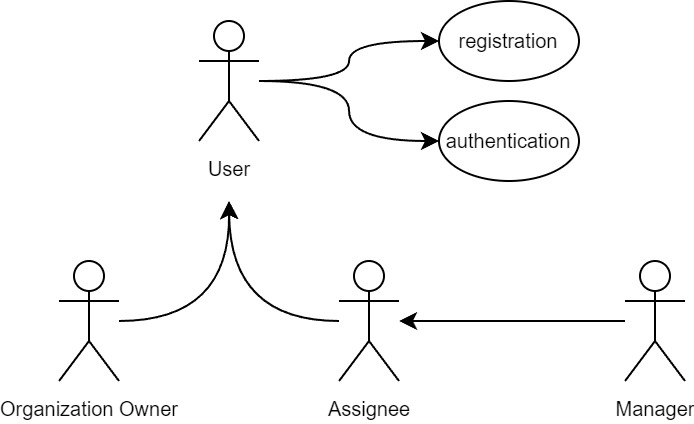
\includegraphics[width=\textwidth, height=\textheight, keepaspectratio]{images/UseCaseDiagram/UseCaseUser.jpg}
\subsection*{Description}
In our system, a critical part is the registration and the following authentication. This concept keeps valid for every kind of user withing the platform.
In the system, 3 type of user are made available.
The most important one is the Organization Owner. It is responsible of deploying the entire organization and managing every user contained in it. More of that will be discussed later.
The other roles are the Assignee and the Manager. The assigne is considered to be the last in the logistic chain, responsible for completing tasks and managing its own notes for the AI report system to work.
Finally, the Manager actor inherits everything from the assignee, but he is granted some major capabilities, such as managing tasks, creating subtasks and all things related to them.
\subsection{Authentication structure}
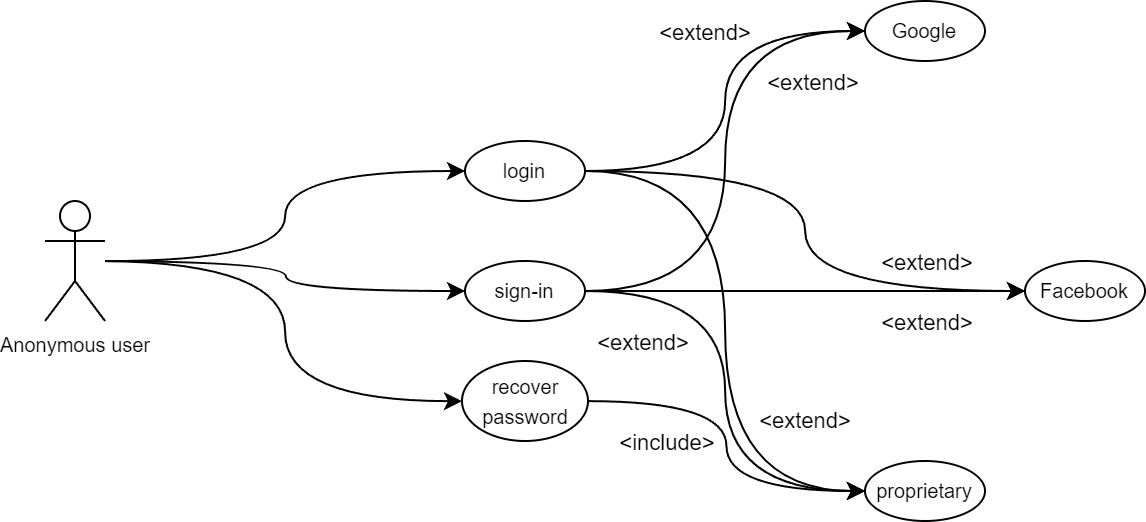
\includegraphics[width=\textwidth, keepaspectratio]{images/UseCaseDiagram/UseCaseAuthentication.jpg}
\subsection*{Description}
There are multiple methods for end-users to access the platform. Initially, users can utilize Google and Facebook APIs, which allow them to conveniently access the platform using their existing accounts. Additionally, a proprietary system for account creation and management will be provided.\\
Here is the authentication structure flow:
\begin{itemize}
    \item  An anonymous user initiates a login request.
    \item A subsequent sign-in request is made, utilizing the sign-in APIs mentioned above.
    \item  Once authenticated, the user is granted access to the platform.
\end{itemize}
In the event that a user forgets their credentials, a password recovery system will be available. This system will send an email to the user containing a recovery link.
\subsection{Owner structure}
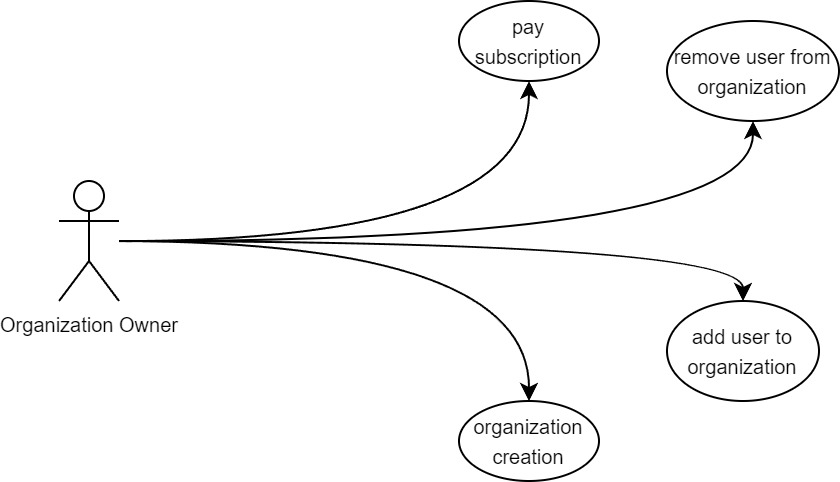
\includegraphics[width=\textwidth, keepaspectratio]{images/UseCaseDiagram/UseCaseOwner.jpg}
\subsection*{Description}
The organization owner holds full system capabilities. It is their responsibility to add and remove users, as well as create the organization itself. They are also tasked with paying the subscription for the service, calculated based on the platform usage rate and managed through external banking APIs.\\
More of that will be discussed in later sections.
\subsection{Assignee and Manager structure}
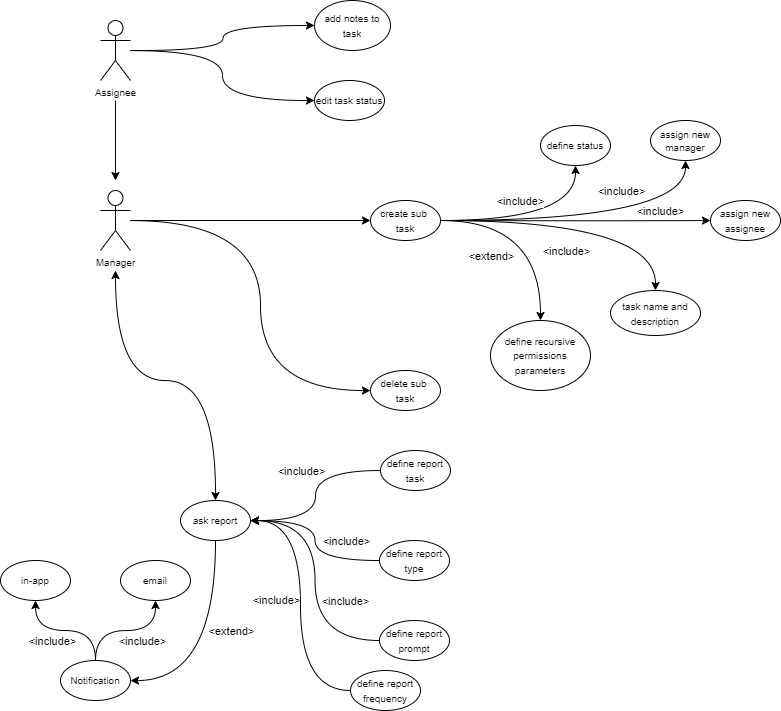
\includegraphics[width=\textwidth, keepaspectratio]{images/UseCaseDiagram/UseCaseAssigneeManager.jpg}
\subsection*{Description}
As an assignee, my primary responsibility is to add notes and edit task statuses based on the daily workload. Additionally, a manager also has the permission to create subtasks.

This critical aspect involves several components:
\begin{itemize}
\item Definition of the status (modifiable during the lifecycle of the subtask).
\item Nomination of the manager, as well as the assignees.
\item Definition of recursive permission parameters (further details below).
\item Naming and description of the task.
\end{itemize}

Managers also have the permission to delete subtasks, whether completed or not.

Furthermore, managers gain the capability to request a report. This request should include details such as the inquiring task, its type (AI-managed or not), its prompt, and its frequency. The notification system will inform the targeted users via email or in-app notification.
%VERIFICARE CONGRUENZA TRA I 2

\section{Context Diagram}
This section illustrates the context diagram of the system and describes the relations between MindMerge and two different kinds of external entities.

\subsection{Diagram}
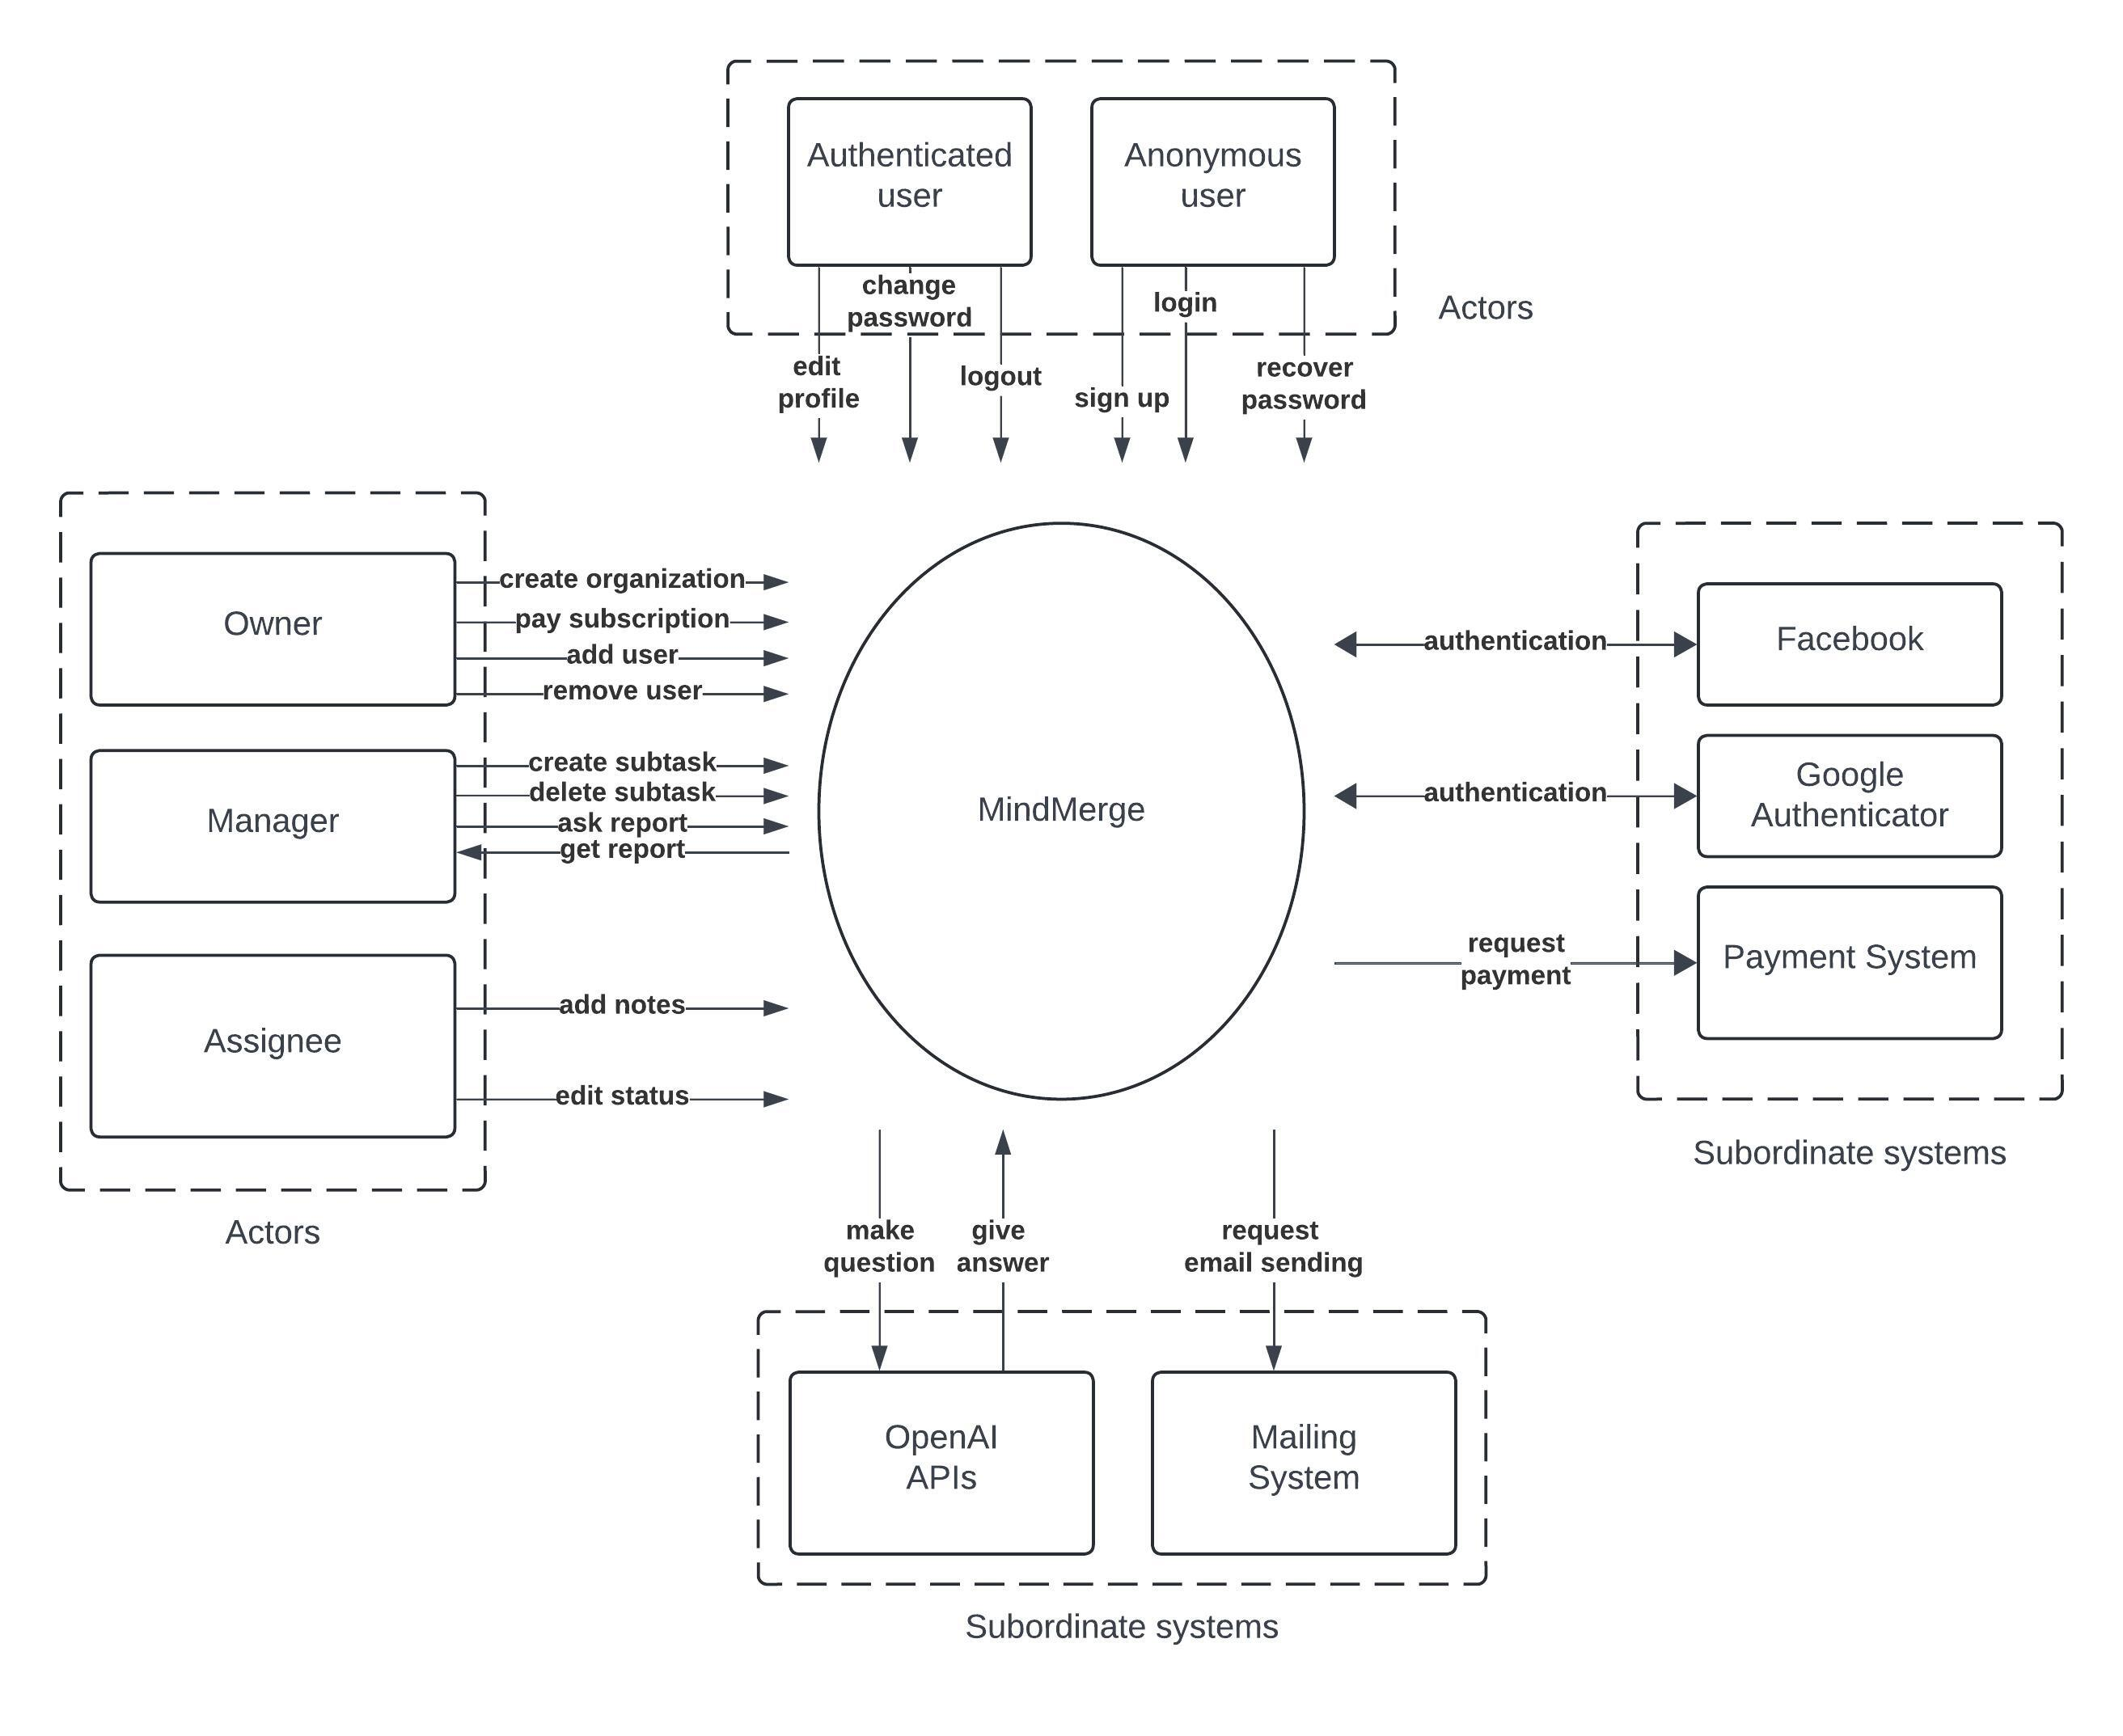
\includegraphics[width=\textwidth, height=\textheight, keepaspectratio]{images/context_diagram.jpeg}

\subsection{Subordinate systems}
External softwares that are used by MindMerge to provide services to the users.
\begin{itemize}
    \item Google Authenticator and Facebook: they are used to give to users the possibility to log in using their Google or Facebook account. Allowing third party authentication, the system doesn't force user to create a new MindMerge account.
    \item Payment System: it is used to allow Organization's owner to pay for the system's subscription.
    \item OpenAI APIs: they are used, on manager request, to generate an automatic report of job done by assignees. MindMerge requests a report to the APIs and is given back the result.
    \item Gmail: it is used as part of the notification system to notify creation of new tasks or updates to the existing ones via mail.
\end{itemize}

\subsection{Actors}
Users that interact with the system and are able to use some of its functionalities.
\begin{itemize}
    \item Anonymous user: A user that has not yet authenticated into the system. He is able to access login functionalities, also by using subordinate systems provided for that, to sign up in case he doesn't have an existing account or to recover password in case he isn't able to remember it.
    \item Authenticated user: A user that has completed authentication procedure and is logged into the system. He has the possibility to logout in every moment, becoming an anonymous user, but also to edit his profile or change password.
    \item Owner: A user that is the head of a specific organization. He has the possibility to create an organization, pay the subscription using the external payment system and add or remove users to or from that. He is himself a manager and an assignee, so he also has all the possibilities related to these roles.
    \item Manager: A user that manages a specific task. He has the possibility to create subtasks and doing some operations related to that (define task's status, assign new manager or new assignes to it, defining it's name, description and recursive permission parameters). He is also able to delete the subtasks he has created or to ask and receive reports, that can be generated automatically by using OpenAI APIs or manually by an assignee. He is himself an assignee, so he also has all the possibilities related to that role.
    \item Assignee: A user that is required to complete a specific task by a manager. He has the possibility to edit the task's status, to notify the manager that he has done something he was asked to do, or to add notes, in order to communicate something related to what he did.
\end{itemize}

\section{Components Diagram}

This section illustrate the component diagram of the system. To improve readability we split the components into several sub
components.
Each sub component has a color assigned to it, and the interfaces that are provided by that specific component are painted with the same color.
This helps to quickly identify which component is responsible for a specific interface.
\newline \newline
The list of sub components is the following:
\begin{itemize}
    \item \textcolor[HTML]{8CC86E}{\textbf{Data Base Manager: }} This component is responsible for managing the data base, it is an interface between
          the data base and the rest of the subsystems. The color assigned to this component is \textcolor[HTML]{8CC86E}{green}.
    \item \textcolor[HTML]{F0C832}{\textbf{Notification Manager: }} This component is responsible for managing the notifications;
          This means sending notification, and serve the data to the front end to visualize the pending notification of a user. The color assigned to this component is \textcolor[HTML]{F0C832}{yellow}.
    \item \textcolor[HTML]{FF0000}{\textbf{Account Manager: }} This component manage accounts, in particular it handles sign in, log in, account changes and account deletion.
          The color assigned to this component is \textcolor[HTML]{FF0000}{red}.
    \item \textcolor[HTML]{64C8BE}{\textbf{LLM Prompter: }} This component is a simple library that provide an interface to prompt different LLMs. It's objective is to make the
          implementation of the rest of the system agnostic from the specific LLM used. The color assigned to this component is \textcolor[HTML]{64C8BE}{aqua green}.
    \item \textcolor[HTML]{A0C8F0}{\textbf{Task Tree Navigator: }} This component is a simple library with some algorithm to navigate a tree data structure.
          In our specific case the tree represent the tasks and subtasks of an organization. Since this algorithms are used many
          times throughout the system they have been put in a specific component to make them reusable. The color assigned to this component is \textcolor[HTML]{A0C8F0}{light blue}.
    \item \textcolor[HTML]{FA9646}{\textbf{Report Manager: }} This component manage the reports, in particular it is responsible for generating report automatically (using an LLM) or manually (reminding users with a notification that they have to deliver a report).
          The component also allow users to set report schedule, so that the reports generation can be triggered automatically with a customizable frequency.
          The color assigned to this component is \textcolor[HTML]{FA9646}{orange}.
    \item \textcolor[HTML]{FF00FF}{\textbf{Organization Manager: }} This component allow an user to create an organization, or perform some action on his organizations,
          like adding/removing a user, or paying the subscription to use the software. The color assigned to this component is \textcolor[HTML]{FF00FF}{purple}.
    \item \textcolor[HTML]{2682D5}{\textbf{Task Manager: }} This component allow users to interact with the tasks.
          In particular it is responsible to visualize, create, delete and edit tasks inside one organization. The color assigned to this component is \textcolor[HTML]{2682D5}{blue}.
    \item \textbf{Front End: } This component is responsible for the visualization of the data, and the interaction with the user. This component dose not have a specific color assigned to it, since it dose not provide any interface to other components.
    \item \textcolor[HTML]{E68CB4}{\textbf{External APIs: }} All interfaces provided by external APIs in the system (like authentication, payment, etc.) are painted with the color \textcolor[HTML]{E68CB4}{pink}.
\end{itemize}

\subsection{Data Base Manager}
\subsubsection{Diagram}
\begin{center}
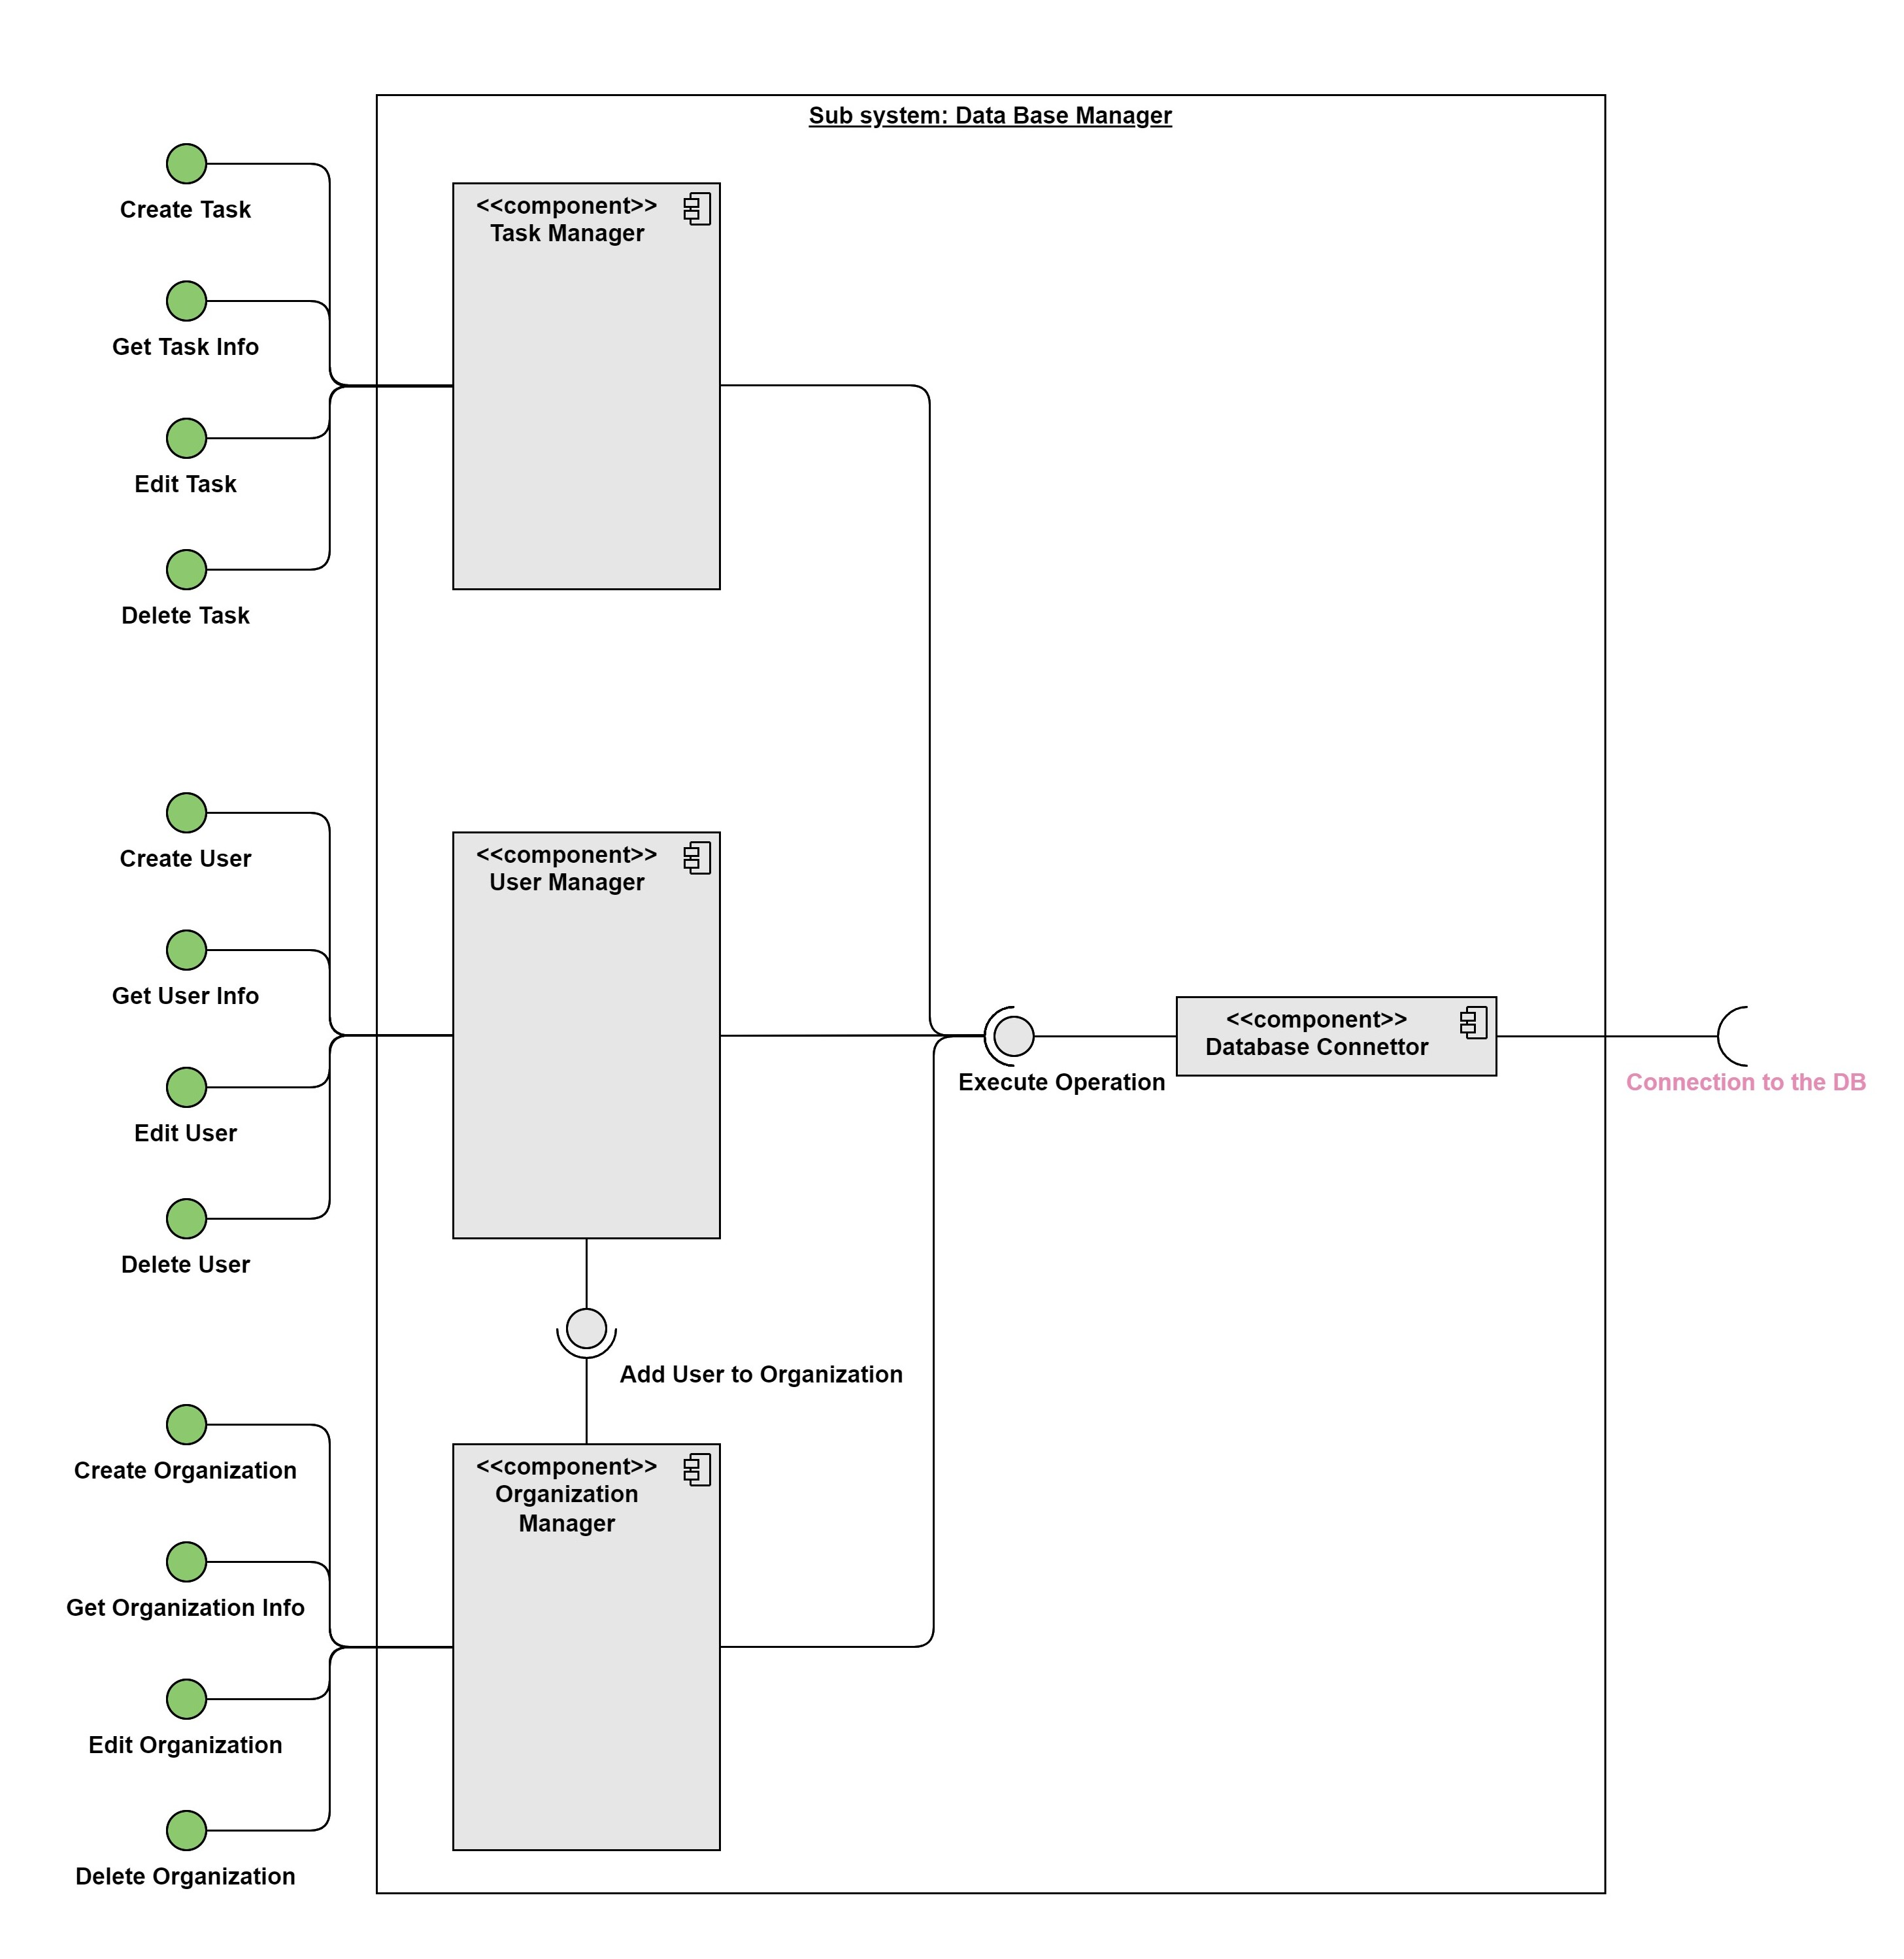
\includegraphics[width=5in,height=\textheight,keepaspectratio]{images/component_diagram/data_base_manager.jpg}
\end{center}
\subsubsection{Descriptions}

We have model the system with 3 particular objects (tasks, users and organizations).
The database manager has a specific component to manage each one of them. The interfaces provided
are divided fot the kind of action that needs to be performed (creation, deletion, modification or read operations).

\subsection{Notification Manager}
\subsubsection{Diagram}
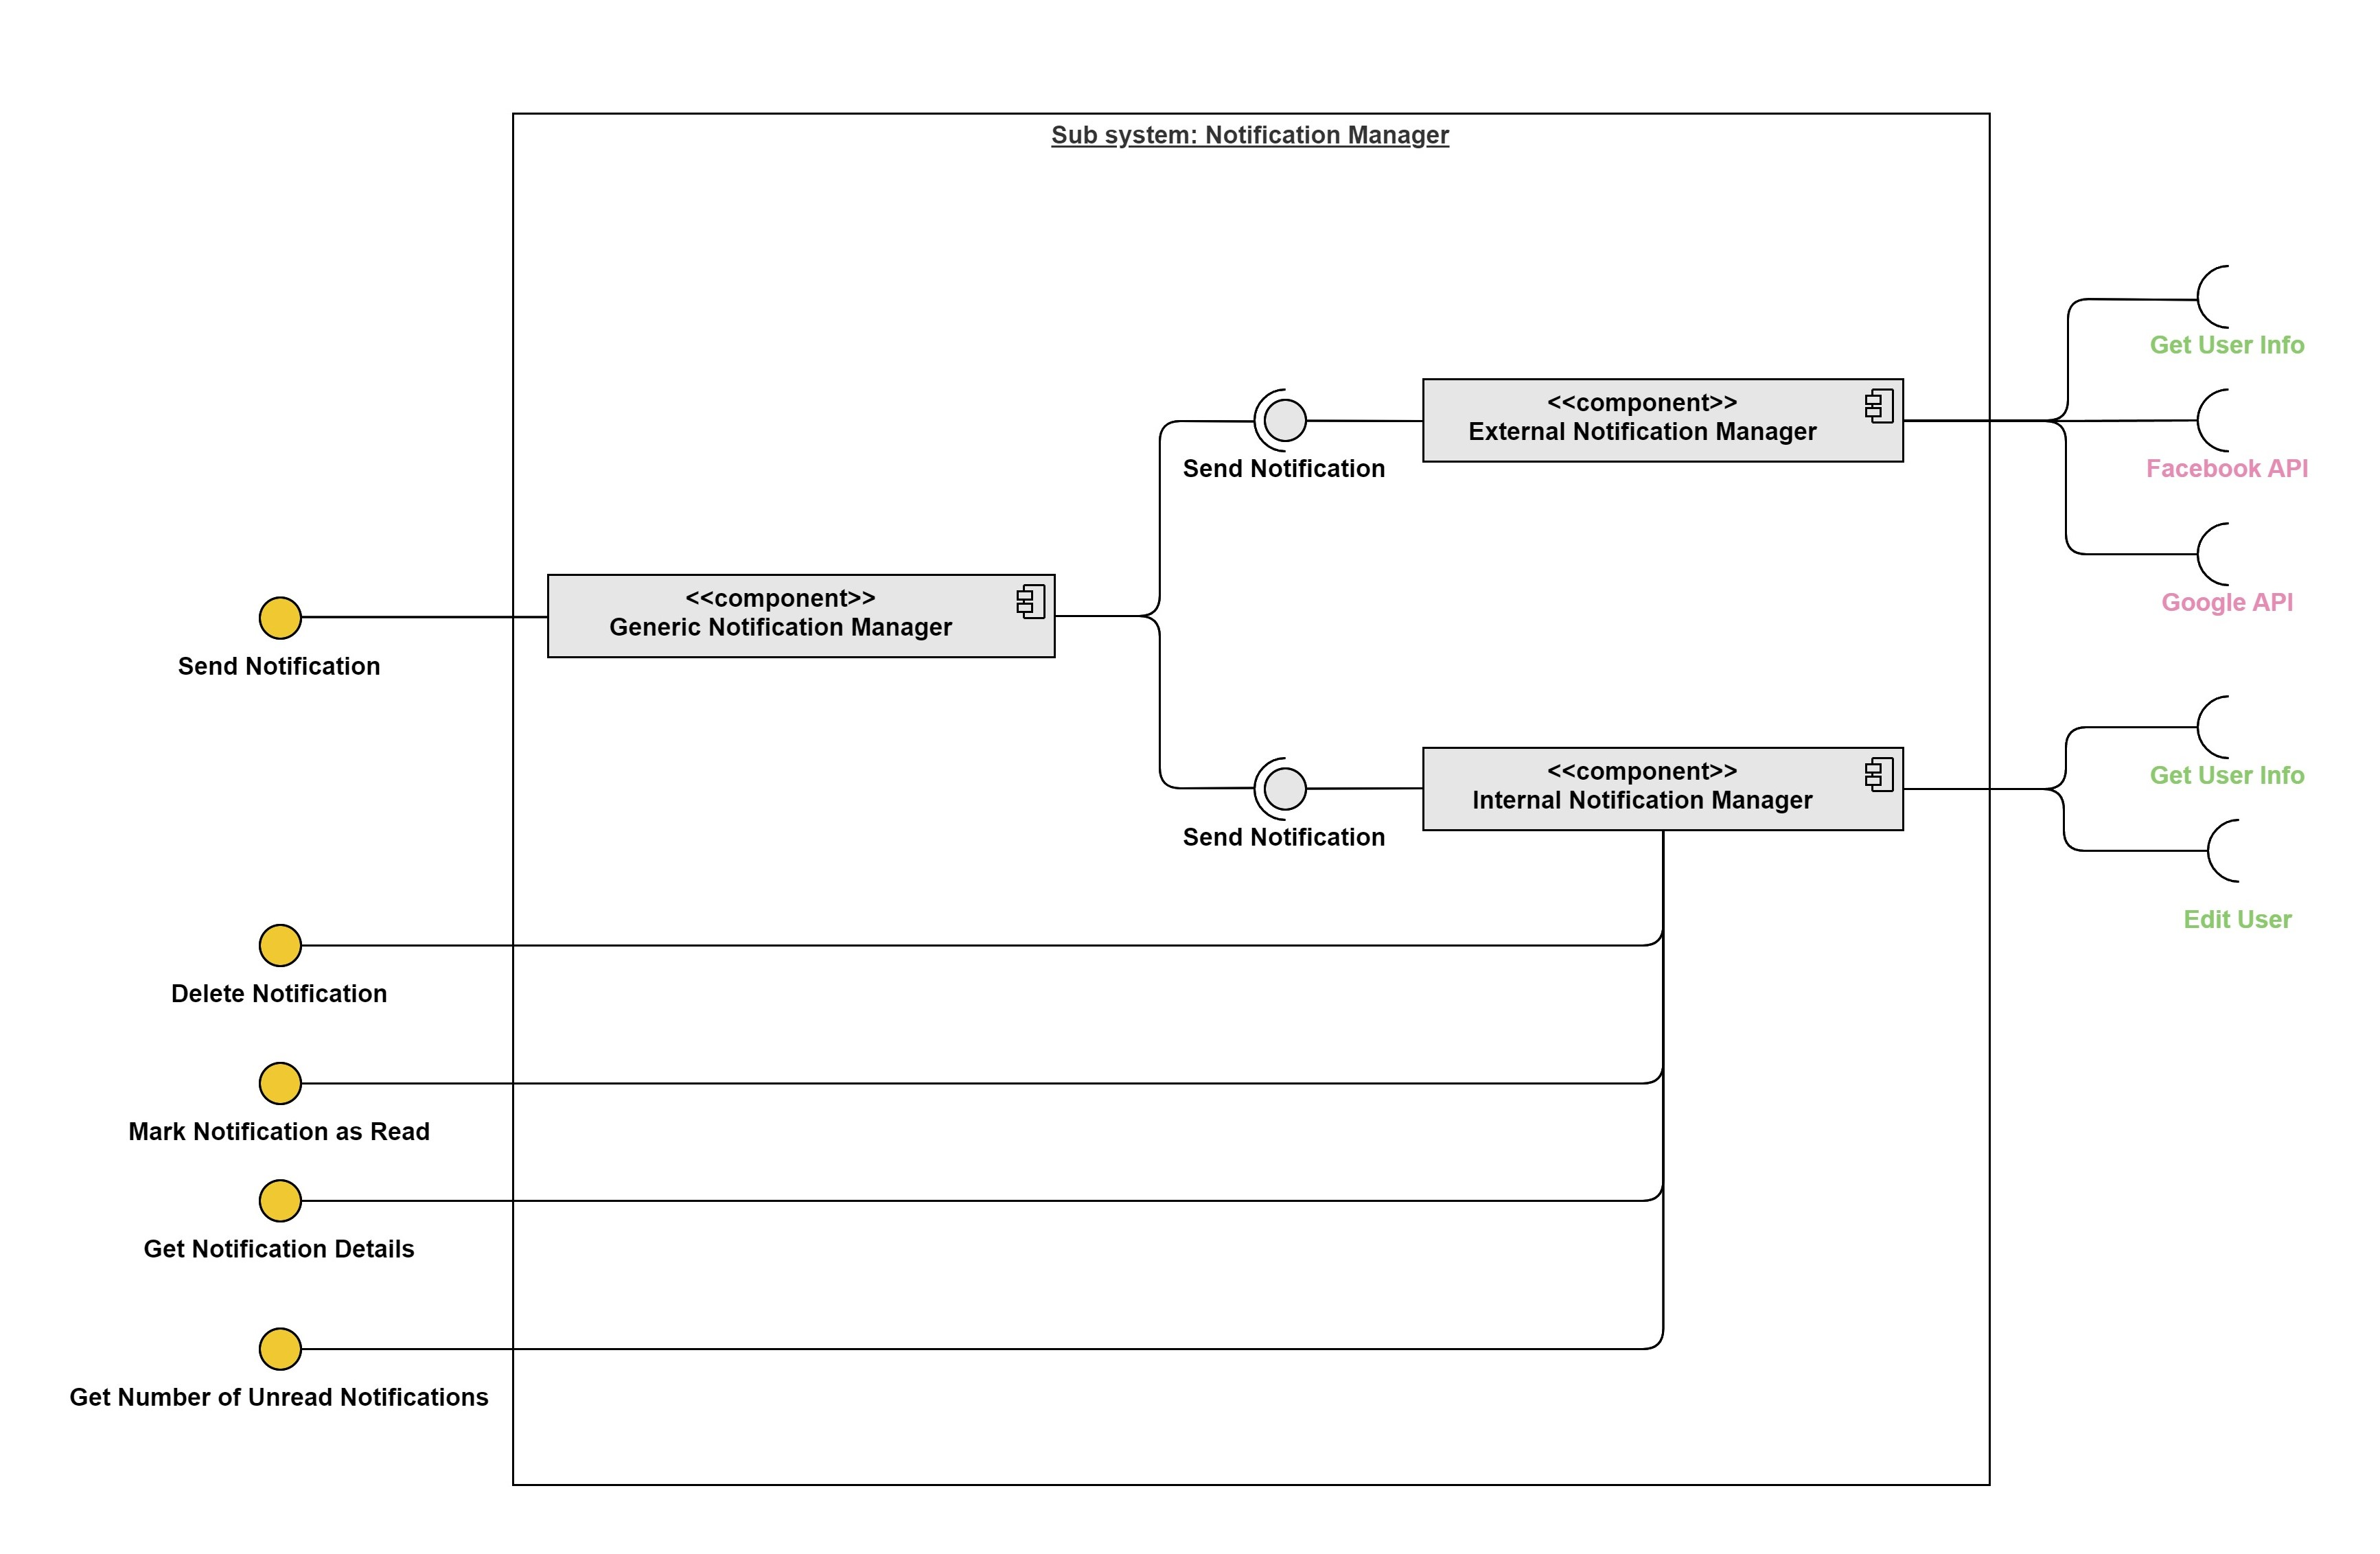
\includegraphics[width=\textwidth,height=\textheight,keepaspectratio]{images/component_diagram/notification_manager.jpg}
\subsubsection{Descriptions}
The notification manager system has 2 specific tasks:
\begin{itemize}
    \item Allowing other components to send notification to users.

          This is done by the ``send notification'' interface
    \item Allow a user to visualize pending notification in the front end

          This id done by the other 4 interfaces
\end{itemize}

The system is composed of 3 different component
\begin{itemize}
    \item \textbf{Generic Notification Manager: }

          This component is the one that provided the ``Send Notification'' interface, and it only act as
          a switch. The system allow for notification to be sent either via mail, or with an in-app notification.
          When a notification comes in to be send this component will decide where to send it.
    \item \textbf{External Notification Manager: }

          This component will send a mail with a notification to a specific user.
          This component has various external APIs connected to it, as how the notification is sent will depend on how the user signed In.
    \item \textbf{Internal Notification Manager: }

          This component manage the in-app notifications. It can either be asked to send a notification (in this case it writes it in the database)
          or it can be asked to get a notification by the front end, so that it can be visualized (in this case it reads the necessary data from the database)

\end{itemize}

\subsection{Account Manager}
\subsubsection{Diagram}
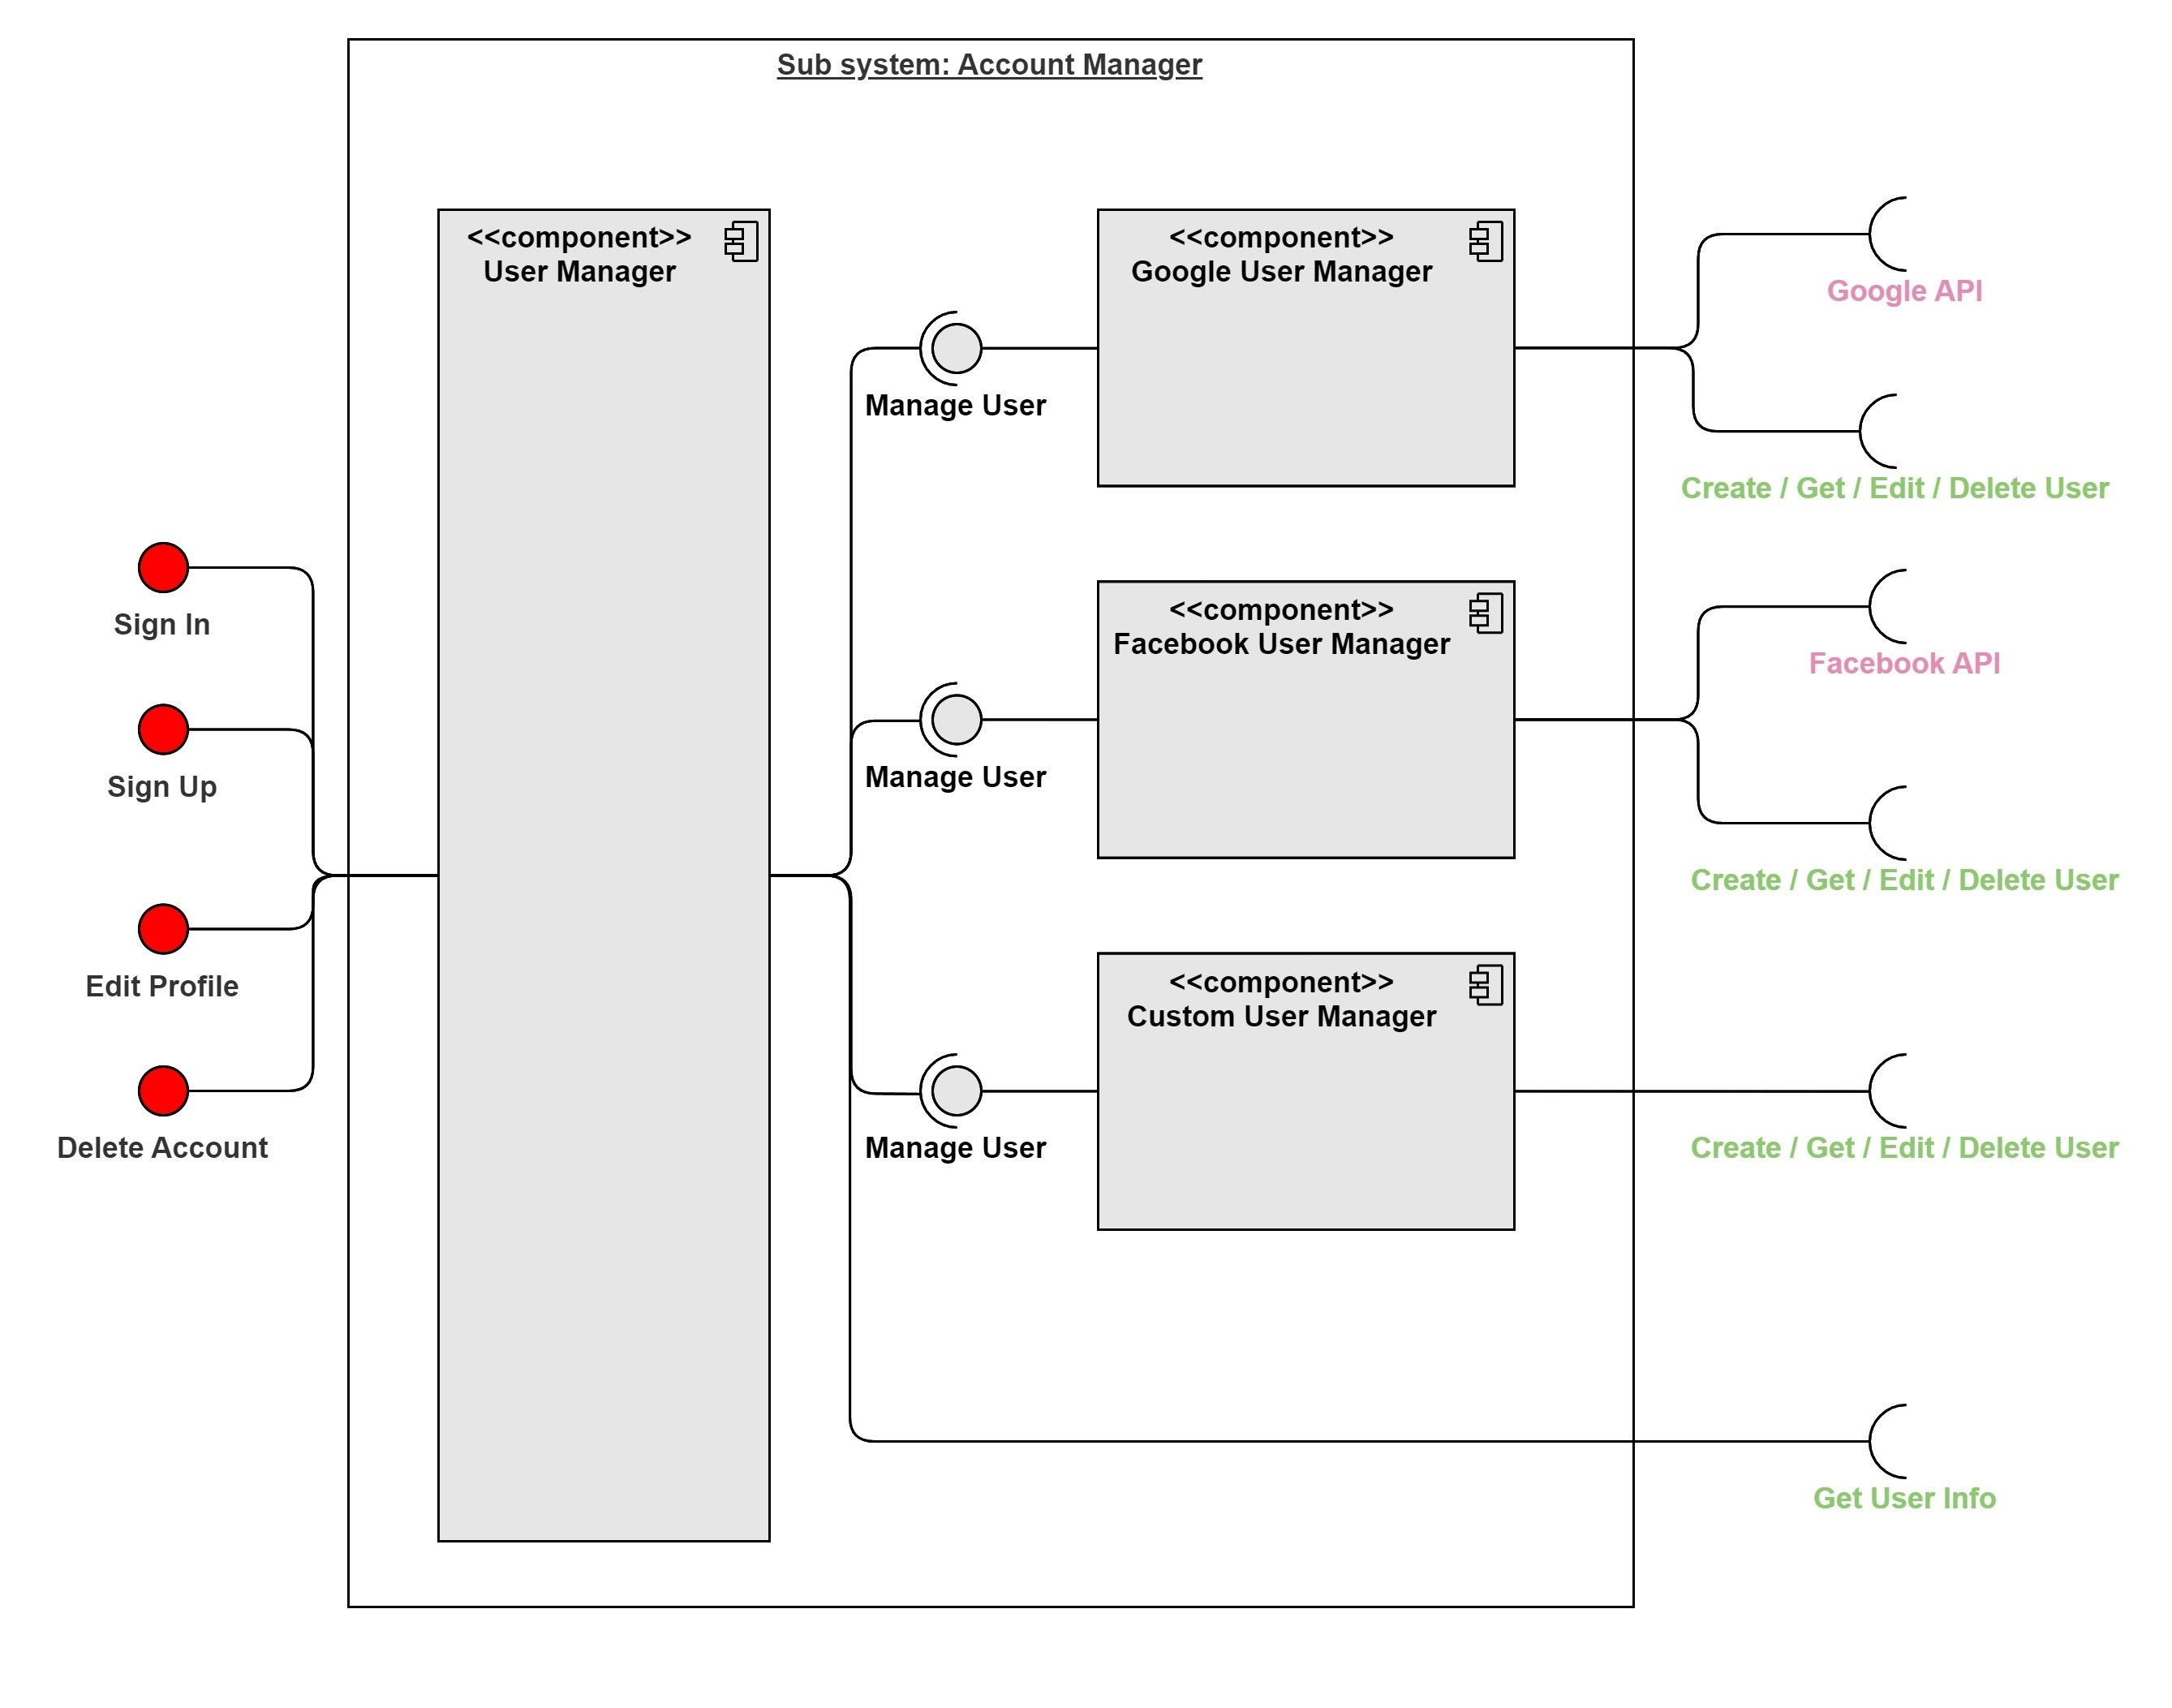
\includegraphics[width=\textwidth,height=\textheight,keepaspectratio]{images/component_diagram/account_manager.jpg}
\subsubsection{Descriptions}
The account manager system allow users to register, log in, delete account and change account information (like password, name, ecc.).

The specific implementation depends on how the user signed in. For this reason the system has a switch component (``User Manager'')
that will decide which specific implementation to use for each specific user. Once this is decided the user
can be handled by one of the 3 components:
\begin{itemize}
    \item \textbf{Google User Manager: }

          This component will handle all the user that signed in with a google account.
    \item \textbf{Facebook User Manager: }

          This component will handle all the user that signed in with a facebook account.
    \item \textbf{Custom User Manager: }

          This component will handle all the user that register with an email and password.
\end{itemize}
Note that we have bundled the database interfaces for managing users into one single interface to enhance readability.
\subsection{LLM Prompter}
\subsubsection{Diagram}
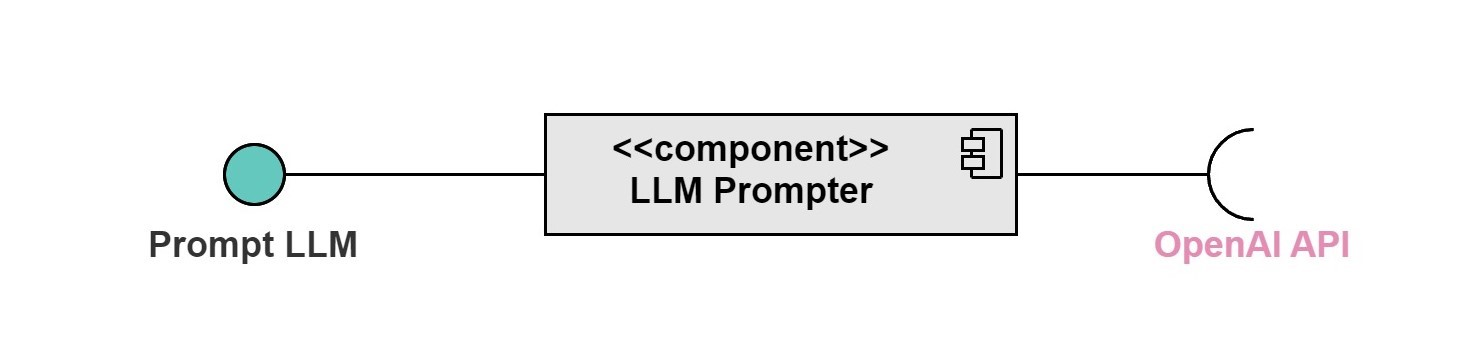
\includegraphics[width=\textwidth,height=\textheight,keepaspectratio]{images/component_diagram/llm_prompter.jpg}
\subsubsection{Descriptions}
This is a simple component that abstract the detail about the specific LLM that is been used from the rest of the system.
This is a good practice that can save some time in the future, if we decide to change the LLM that we are using.
In this example we are using Open AI APIs.

\subsection{Task Tree Navigator}
\subsubsection{Diagram}
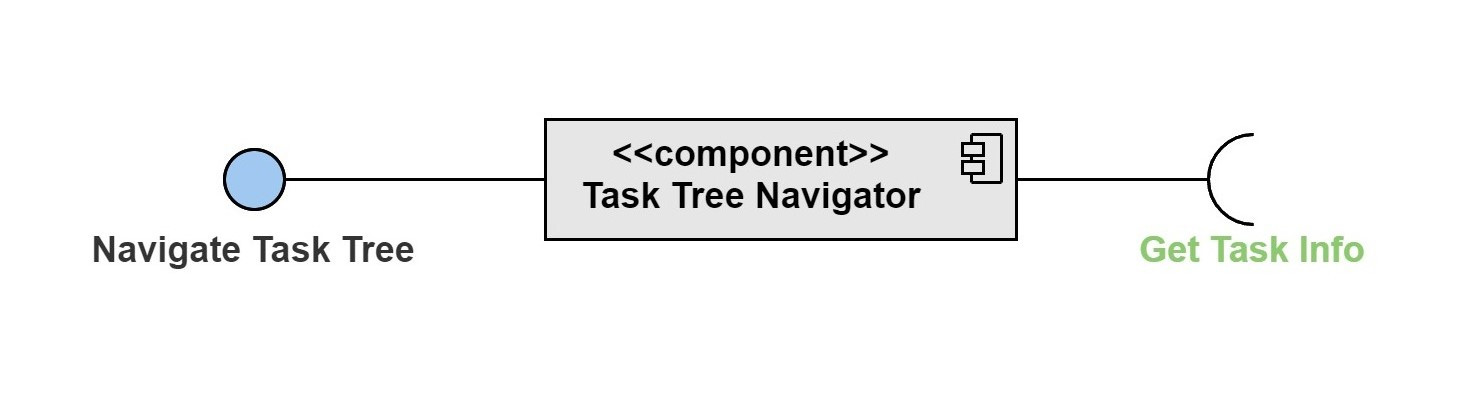
\includegraphics[width=\textwidth,height=\textheight,keepaspectratio]{images/component_diagram/task_tree_navigator.jpg}
\subsubsection{Descriptions}
This component provide some library useful to navigate the task tree. For example it can be used to find all the children of a task, up to a certain depth.

\subsection{Report Manager}
\subsubsection{Diagram}
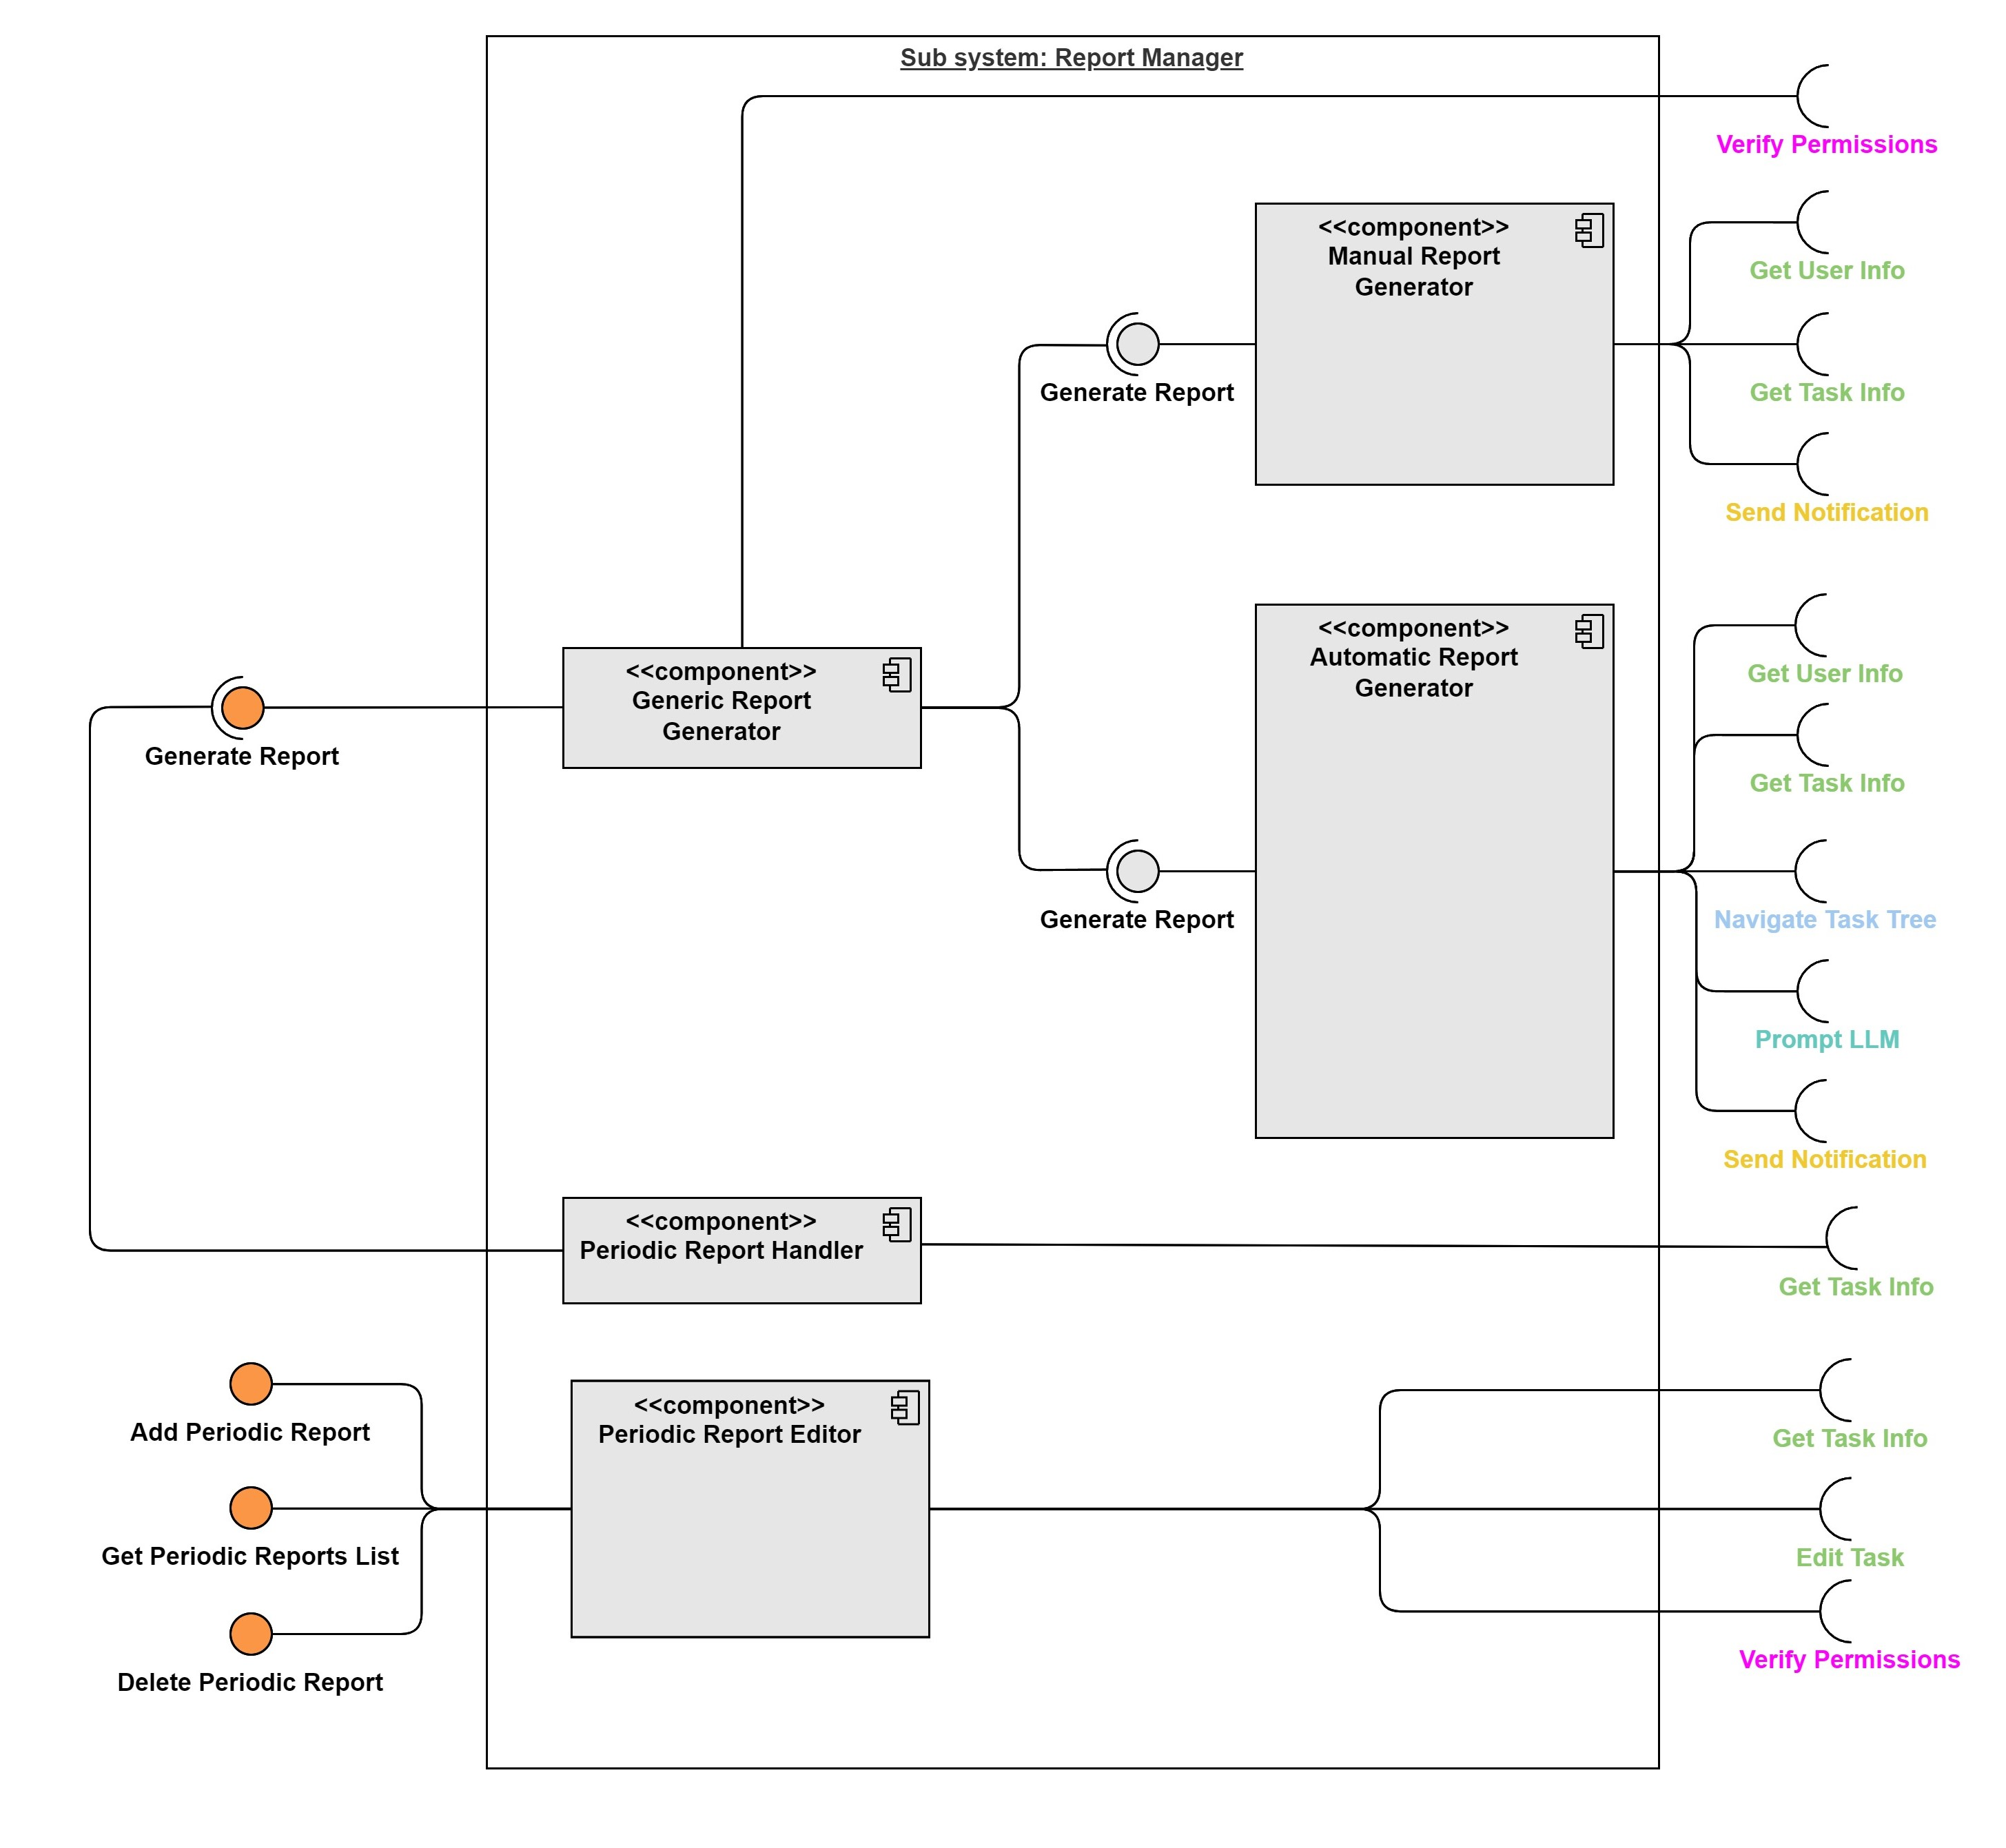
\includegraphics[width=\textwidth,height=\textheight,keepaspectratio]{images/component_diagram/report_manager.jpg}
\subsubsection{Descriptions}
The report manager have two main tasks:
\begin{itemize}
    \item Generating reports (both manually and automatically) 
    \item Managing the report schedule 
\end{itemize}

The system is composed of 5 different components:

\begin{itemize}
    \item \textbf{Manual Report Generator: }

    This component is responsible for generating manual reports. A manual report is a report that ir generated by a user, and not by the system.
    So in practice this component will just remind the user that he has to deliver a report.
    \item \textbf{Automatic Report Generator: }

    This component is responsible for generating automatic reports. An automatic report is a report that is generated ry the system,
    using an LLM. This component will use some LLM APIs, as well as the data that it could find in the database to generate the report, and then it will deliver It
    to the user how requested it, using the notification system.

    \item \textbf{Generic Report Generator: }
    
    This component is the one that provided the ``Generate Report'' interface, and it only act as a switch, That 
    will forward the request to the correct component (manual or automatic report generator).
    The component also verify that the user has the permissions to ask for the report

    \item \textbf{Periodic Report Editor: }

    This component is responsible for managing the report schedule.
    It will allow users to set the frequency of the scheduled reports, as well as to edit or delete them.
    Every time an operation is requested this component will verify the user's permission before executing the request.

    \item \textbf{Periodic Report Handler: }
    
    This component is responsible for handling the scheduled reports.
    It will read the schedule from the database, and then it will trigger a report generation event when the time comes.

\end{itemize}

\subsection{Task Manager}
\subsubsection{Diagram}
\begin{center}
    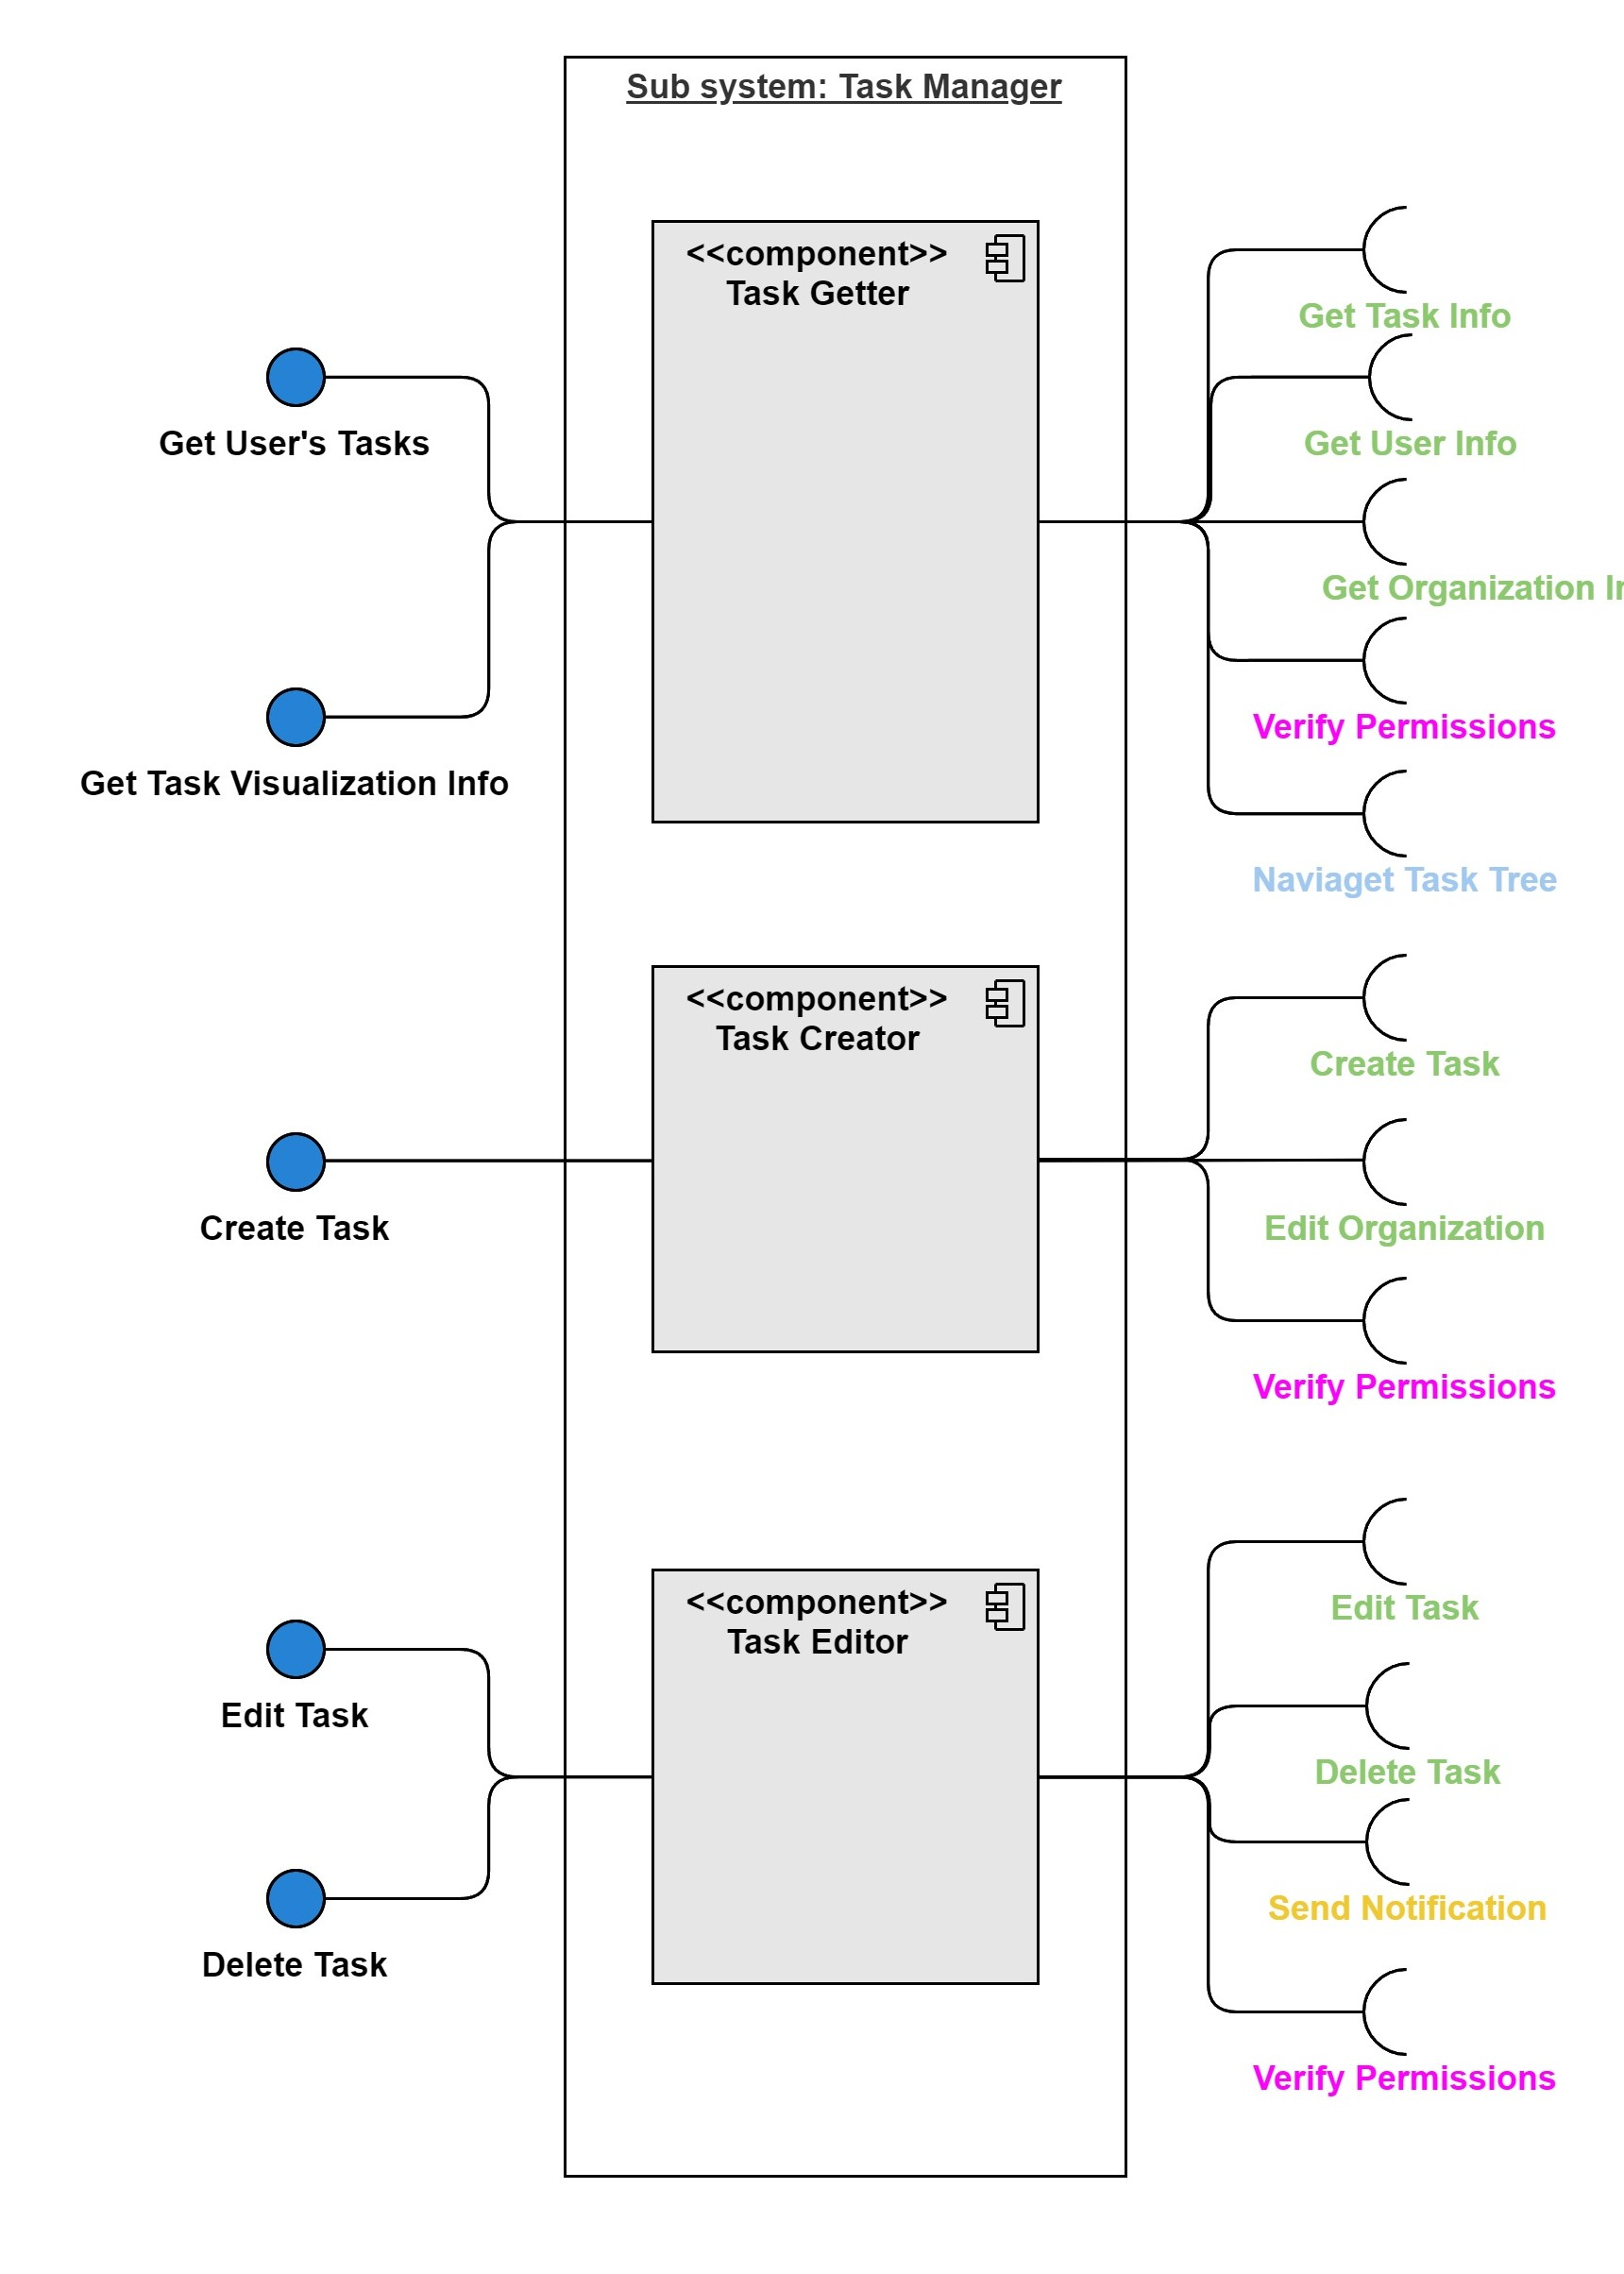
\includegraphics[width=5.5in,keepaspectratio]{images/component_diagram/task_manager.jpg}
\end{center}
\subsubsection{Descriptions}

The task manager is the component that allow users to interact with the tasks.
The interaction are divided in 3 main categories:
\begin{itemize}
    \item \textbf{Task Creation: }
    This is the process of creating a new task. That include operations like 
    setting the task name, the father task, the assignees, the managers ecc.
    This operations are handled by the ``Task Creator'' component.
    \item \textbf{Task Modification: }
    This is the process of modifying an existing task. That include operations like adding a descriptions or some notes,
    changing state, deadline assignee ecc; or even deleting the task.
    This operations are handled by the ``Task Editor'' component; This component will also send a notification to the manager of the task
    if the notification are enabled for the particular task.
    \item \textbf{Task Reading Operation: }
    This process is responsible for reading the task data from the database, and then serve it to the front end.
    This operations are handled by the ``Task Getter'' component.
\end{itemize}


\subsection{Organization Manager}
\subsubsection{Diagram}
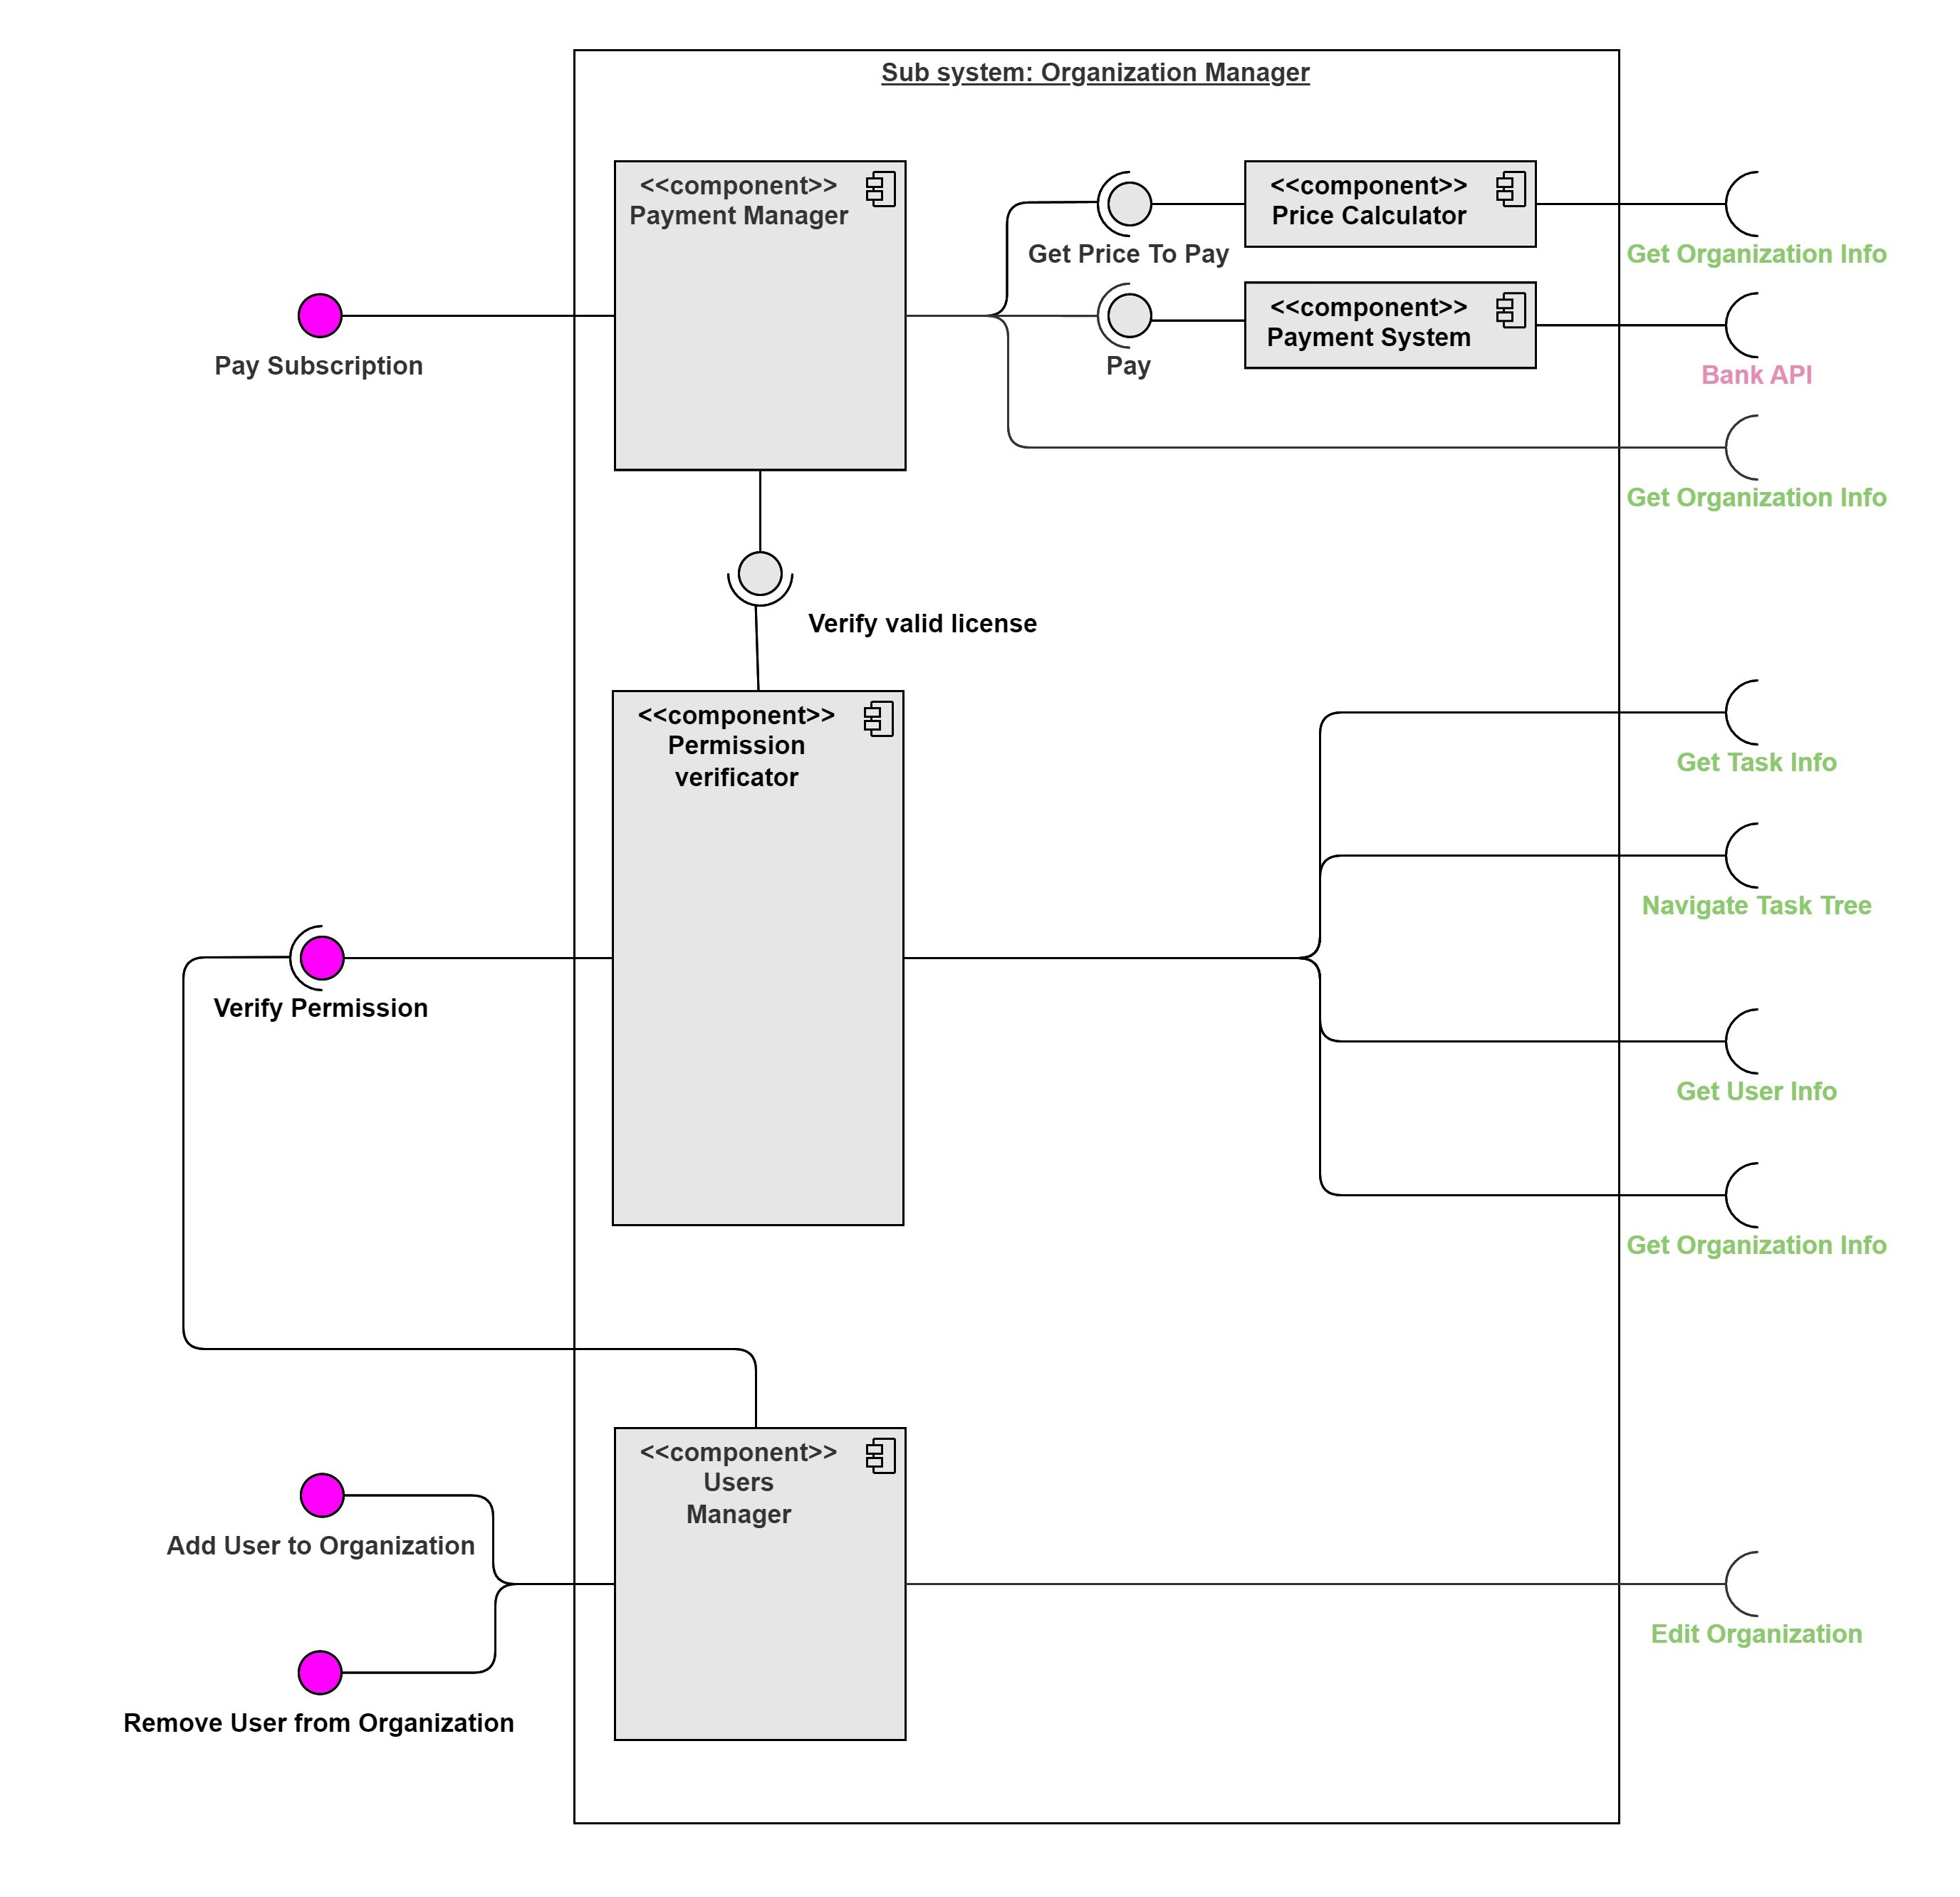
\includegraphics[width=\textwidth,height=\textheight,keepaspectratio]{images/component_diagram/organization_manager.jpg}
\subsubsection{Descriptions}

The organization manager has 3 main tasks:
\begin{itemize}
    \item \textbf{Allowing the manager to pay a subscription}

    The manager should be able to pay the subscription of our software, this is done by the component ``Payment Manager''.
    The component has 2 subordinate components:
    \begin{itemize}
        \item \textbf{Price Calculator: } This component calculate the price the owner should pay based on the number of users in the organization
        \item \textbf{Payment System: } This component is used to connect with the necessary banking system to handle payments
    \end{itemize}

    \item \textbf{Permission Verificator}

    This component is responsible for allowing or denying users actions. it will consider the permissions set in the task by connecting to the database,
    and it will also consider the validity of a license, so we can limit certain actions if the owner hasn't renewed the subscription.

    \item \textbf{User Manager}
    
    This component is the one that will allow an owner to add or remove users form his organization.
\end{itemize}


\subsection{Front End}
\subsubsection{Diagram}
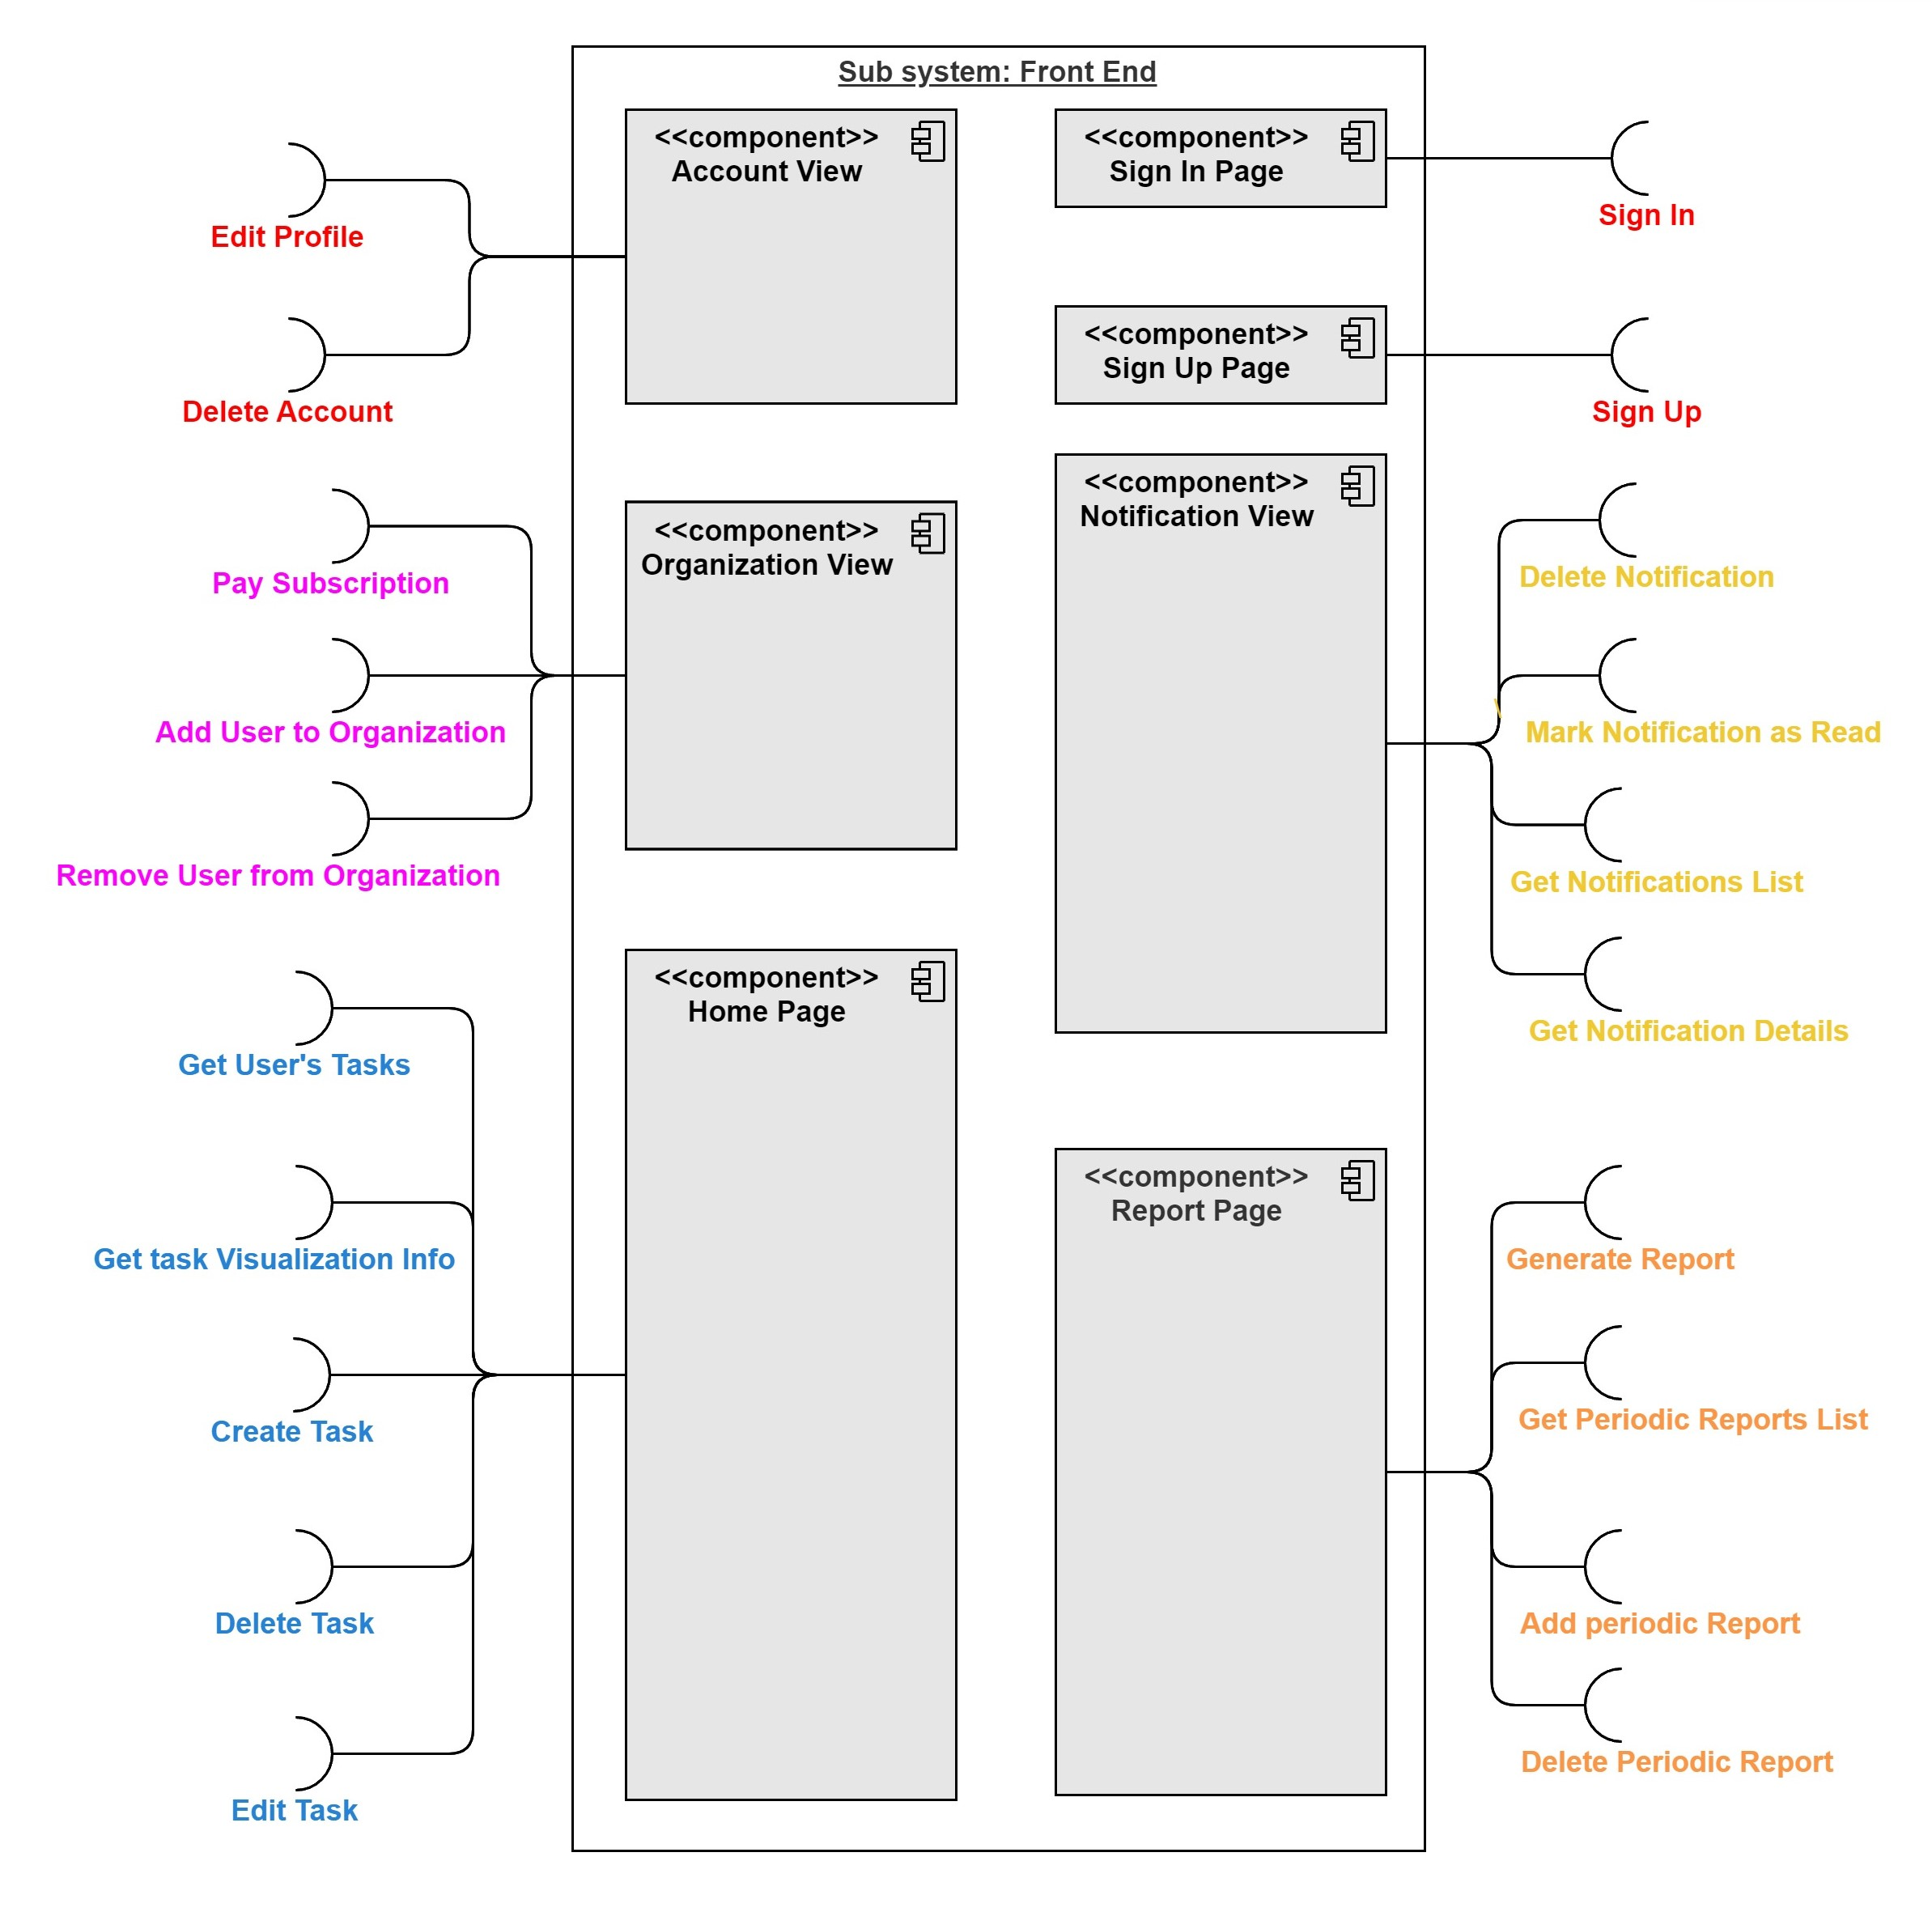
\includegraphics[width=\textwidth,height=\textheight,keepaspectratio]{images/component_diagram/front_end.jpg}
\subsubsection{Descriptions}
In the front end diagram we decided to create one component for every page of the application, for a total of 7 components:
\begin{itemize}
    \item \textbf{Sign In Page: } In this page the users will be able to sign in to the application.
    \item \textbf{Sign Up Page: } In this page the users will be able to sign up for the application
    \item \textbf{Home Page: } This is the main page of the application, where the user will be able to see/edit/create all the tasks of the organization.
    \item \textbf{Report Page: } This page will allow users to ask for a report, or set up a Periodic Report.
    \item \textbf{Notification View: } This page will allow users to see all the pending notifications.
    \item \textbf{Organization View: } This page will allow the organization owner to manage the organization, including things like adding/removing users, or paying the subscription.
    \item \textbf{Account View: } This page will allow the user to manage his account, including things like changing the password, or deleting the account.
\end{itemize}


\section{Class Diagram}

This section will illustrate the class diagram of the system. The class diagram is a static diagram that shows the structure of the system.
We have divided the class diagram in different modules. Each of them in a separate diagram.

All the class names are preceded by the name of the module they belong to, to avoid confusion.

Some time a class can inherits from a class that is defined in another module, in this case
we have represented the foreign class, with the name and tre dots in the place where attributes and methods should be.

\subsection{Data Transfer Objects}

\subsubsection{Diagram}

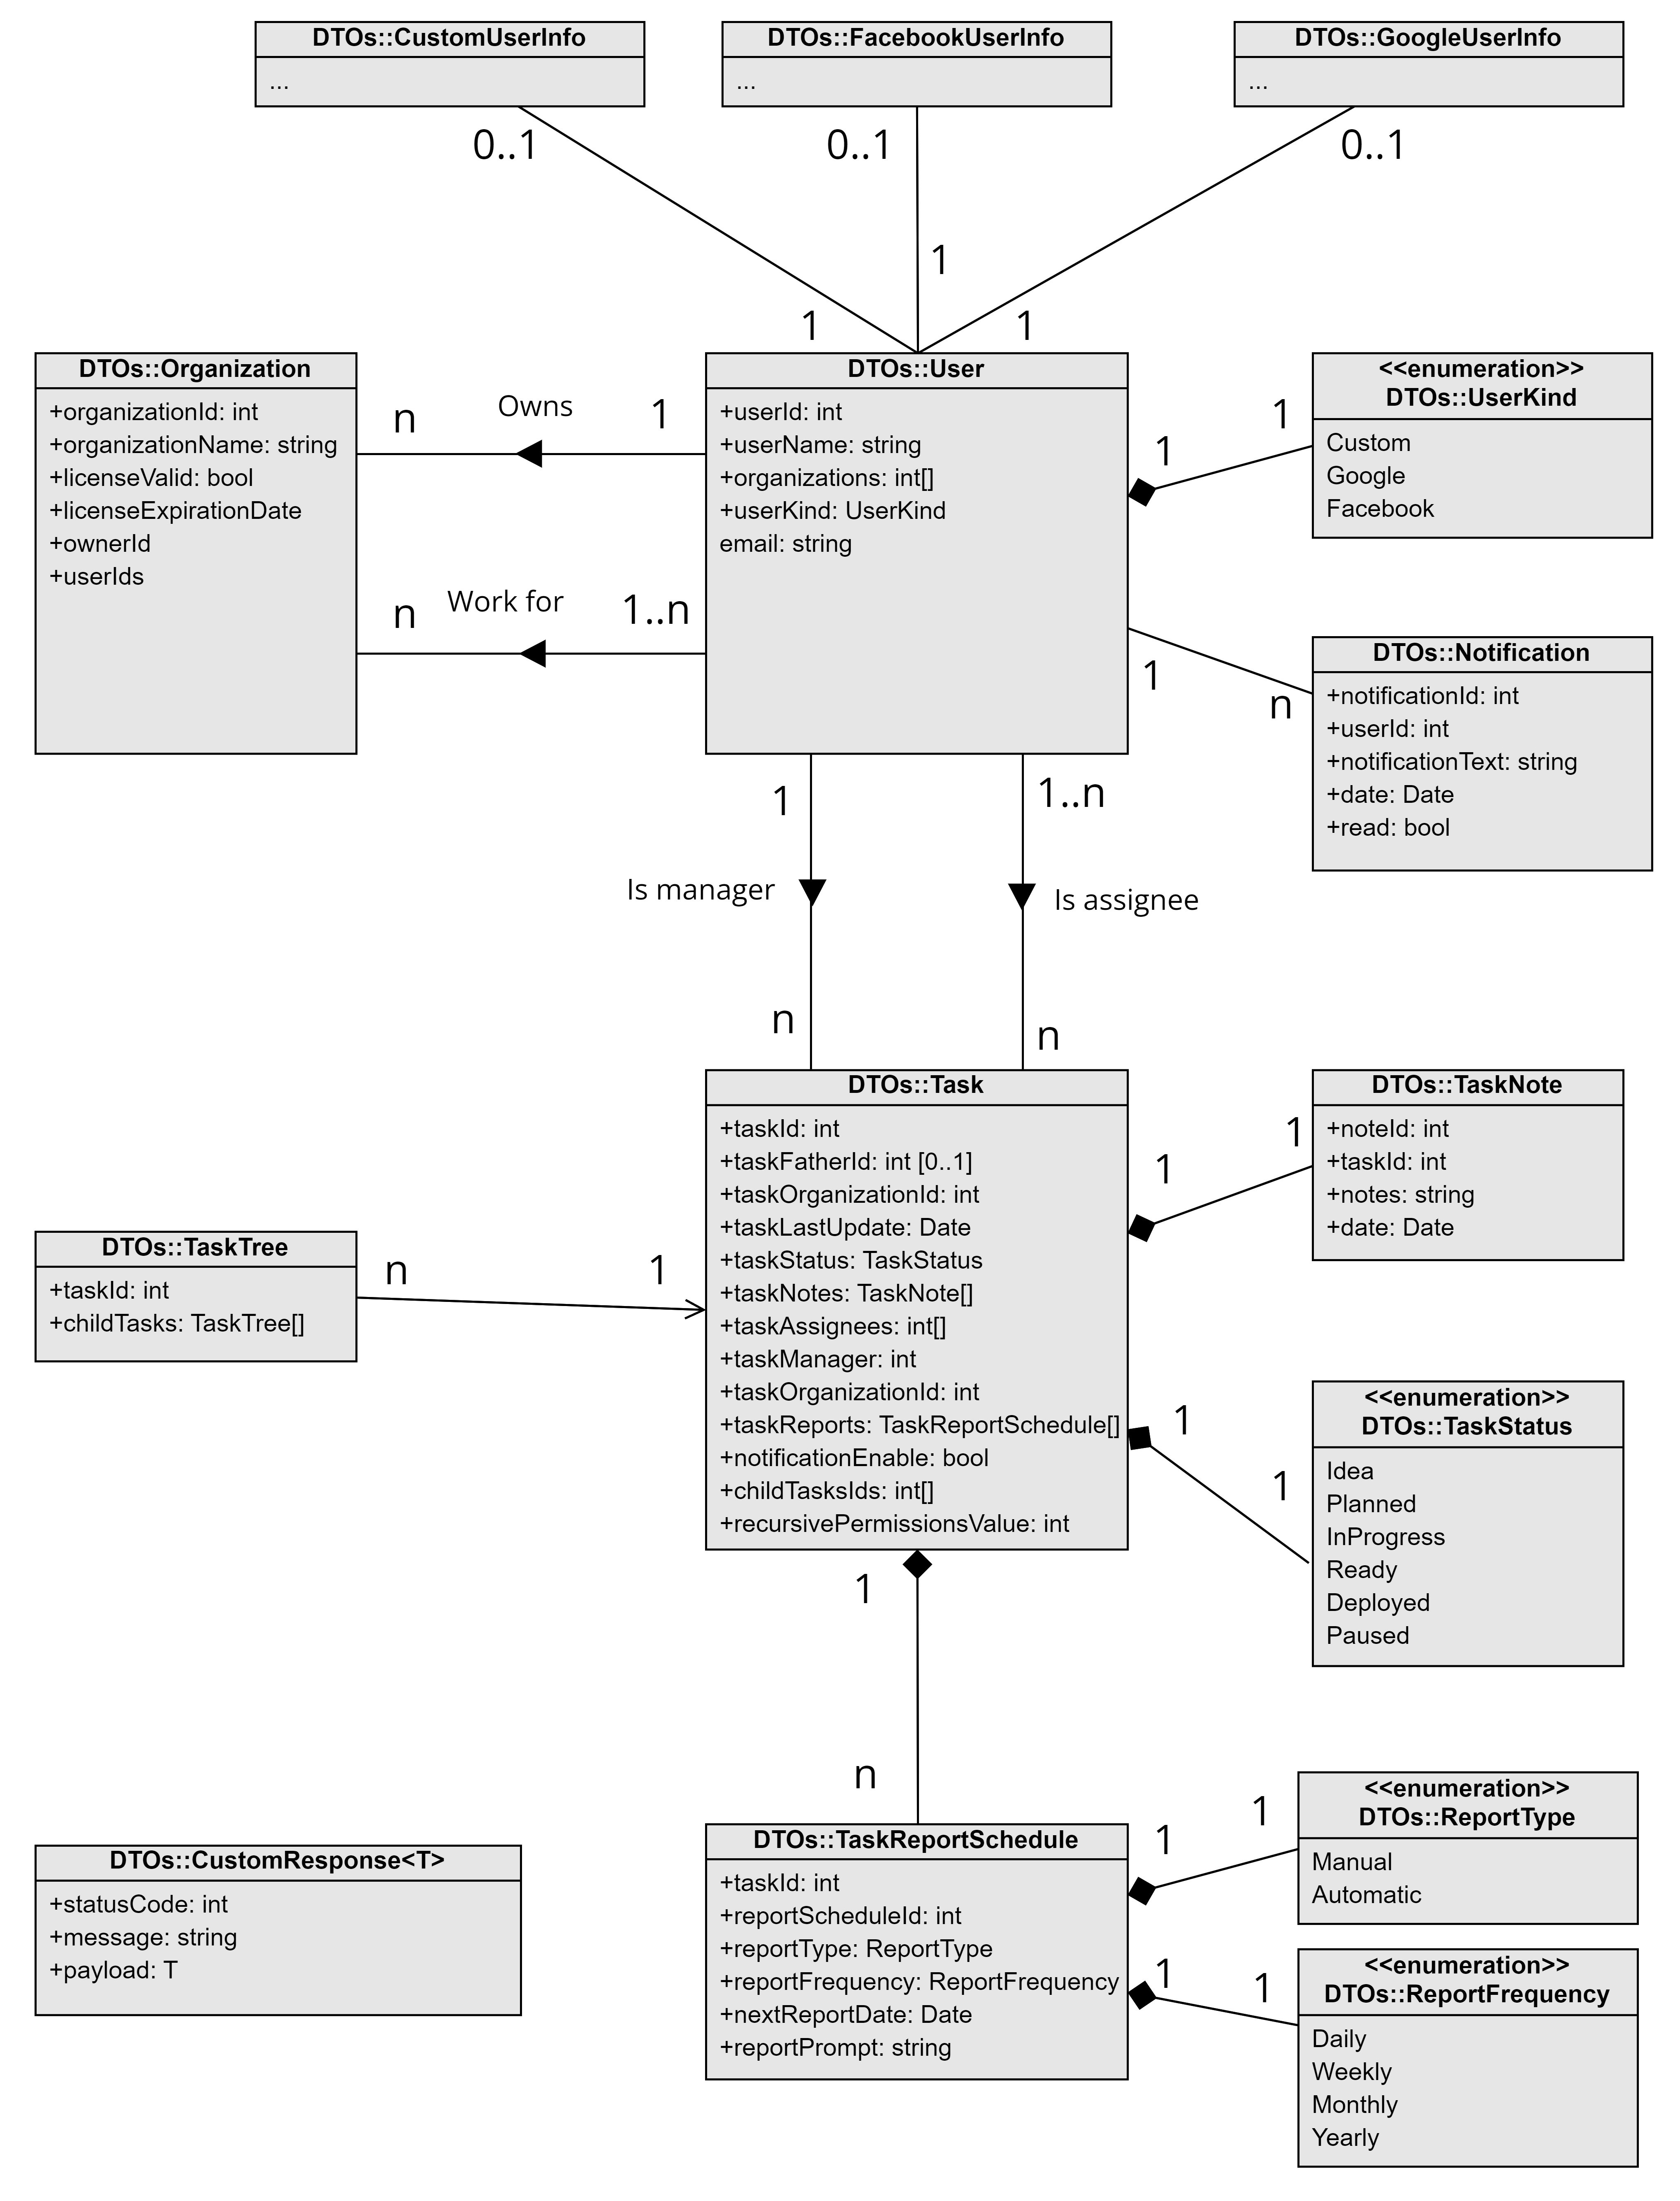
\includegraphics[width=\textwidth,height=\textheight,keepaspectratio]{images/class_diagram/data_transfert_objects.jpg}

\subsubsection{Description}

The data transfer objects (DTOs) are used to represent
all the objects of the system;

In the classes there is a ``Date'' type used, this is an external dependency
from the JavaScript standard library

A list explaining all the classes follows:

\begin{itemize}
    \item \textbf{ReportType: }

    This is an enum that represent the two type of reports that our system can handel: Manual and Automatic.

    \item \textbf{ReportFrequency: }

    This is an enum that represent the various frequency a periodic report can have.

    \item \textbf{TaskReportSchedule: }

    This is a class that represent one report scheduled for a specific day, and with a specific frequency.
    This will be used by the report system to memorize and execute all the scheduled reports.

    \item \textbf{TaskNote: }
    
    This class represent a note that a user add to a specific task.
    A task can have more that one note, and this is represented in the class diagram.

    \item \textbf{TaskStatus: }
    
    This is an enum that represent the various status a task can have.

    \item \textbf{Task: }
    
    This is the class that represent a Task.

    A task has a double associations with users, represent by the two arrows named ``Is manager'' and ``Is assignee''.
    As the associations show, a task must have exactly one manager, and at least one assignee.

    A task is composed of various primitive attributes, like title, task id ecc. 
    And also of some complex attributes, like the a list of \texttt{TaskNotes}, a list of \texttt{TaskReportSchedule} 
    and a \texttt{TaskStatus}. This composition is represented in the class diagram. 

    \item \textbf{TaskTree: }
    
    A Task Tree is a recursive data structure that represent a tree of tasks starting from a root.
    The tree has a root task, and a series of children TaskTree.

    A TaskTree is associated with one task (the root task), this association, is only navigable from the TaskTree to the Task,
    as one task may be associated with more than one TaskTree. This is because
    the visibility of the tasks depends on the user that is looking at the tree.

    \item \textbf{UserKind: }

    This is an enum that represent the various kind of user that can be in the system.
    This derives form the way a user signed in.

    \item \textbf{Notification: }
    
    This class represent a notification issued to a particular user in a specific date.

    \item \textbf{Custom/Facebook/GoogleUserInfo: }
    
    Each user that could have signed in with a different method may require some additionals
    information to be stored in the database. This 3 classes allow us to extend the informations
    of a specific user, depending on how he signed in.

    \item \textbf{User: }
    
    This class represent a user of the system. A user can be linked to some tasks (as manager or assignee),
    and can be linked to some organizations.
    The link to an organization is represented by the association named ``Owns'' and ``Works for''.

    A user is also associated with an unlimited number of notifications, is associated
    with one of the user info between \texttt{CustomUserInfo}, \texttt{FacebookUserInfo} and \texttt{GoogleUserInfo},

    \item \textbf{Organization: }
    
    Thi class represent an organization; And has a double association with users, that represent the owner and the assignees of the organization.

    \item \textbf{CustomResponse}

    This is a class that will be used as a response to all our APIs.
    It will contain a status code, a message and a payload.
    The payload is a generic object represented with the type T
\end{itemize}

\subsection{Data Base Manager} % Gioele

\subsubsection{Diagram}


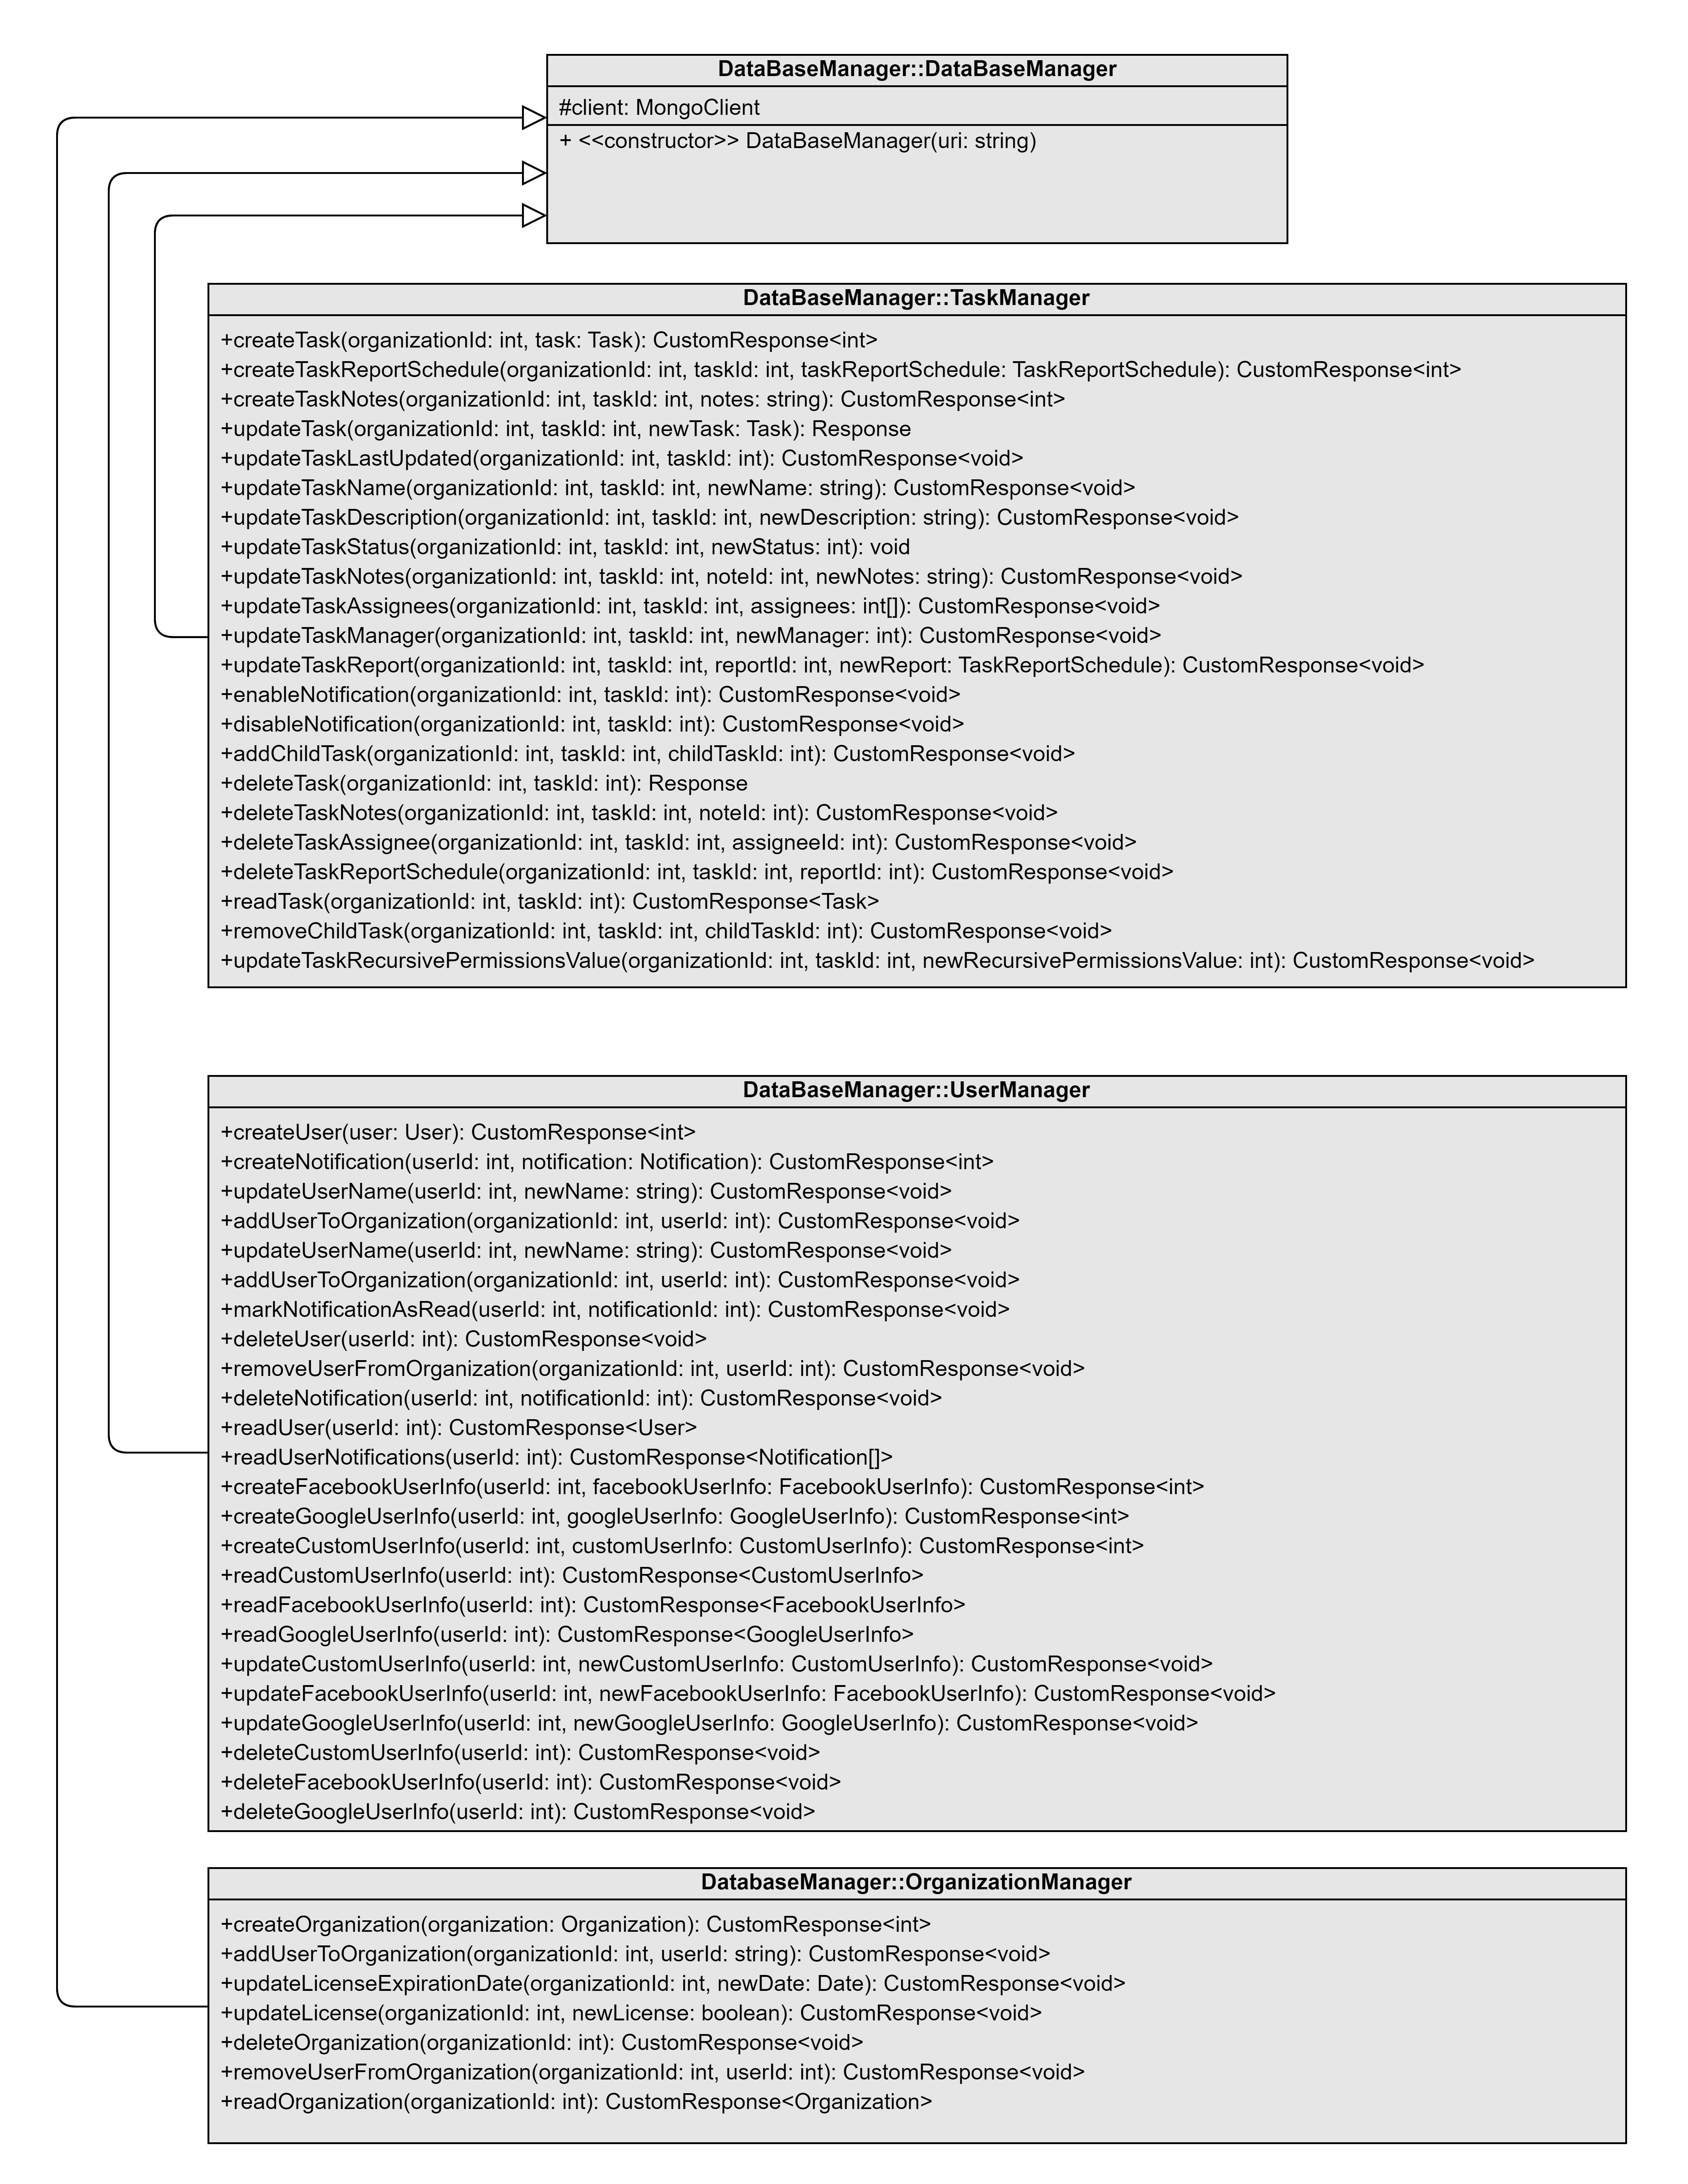
\includegraphics[width=\textwidth,height=\textheight,keepaspectratio]{images/class_diagram/database_manager.jpg}

\subsubsection{Description}

The Data Base Manager is used to store, retrieve and manage every info and object regarding the task, such as the user's notes files and the tasks attributes.
This includes:

\begin{itemize}
  \item \textbf{DataBaseManager: }
  
  A minimalist class containing a constructor only used to instantiate the Mongo driver, required to intercommunicate with MongoDB Atlas.

  \item \textbf{TaskManager: }
  
  A class containing all the methods required for the task system to work. As an instance, That includes methods for the creation, the attributes modification (e.g. report schedule, name) and the subtask management.

  \item \textbf{UserManager: }
  
  A class containg all the methods regarding the user management system. That includes methods to create and update user info, communicate with the external Google and Facebook APIs for authentication and so on.

  \item \textbf{OrganizationManager: }
  
  A class containg all the methods related to the organization itself, managing its creation, deletion and inner user management.

\end {itemize}


\subsection{Services Base Module}

\subsubsection{Diagram}

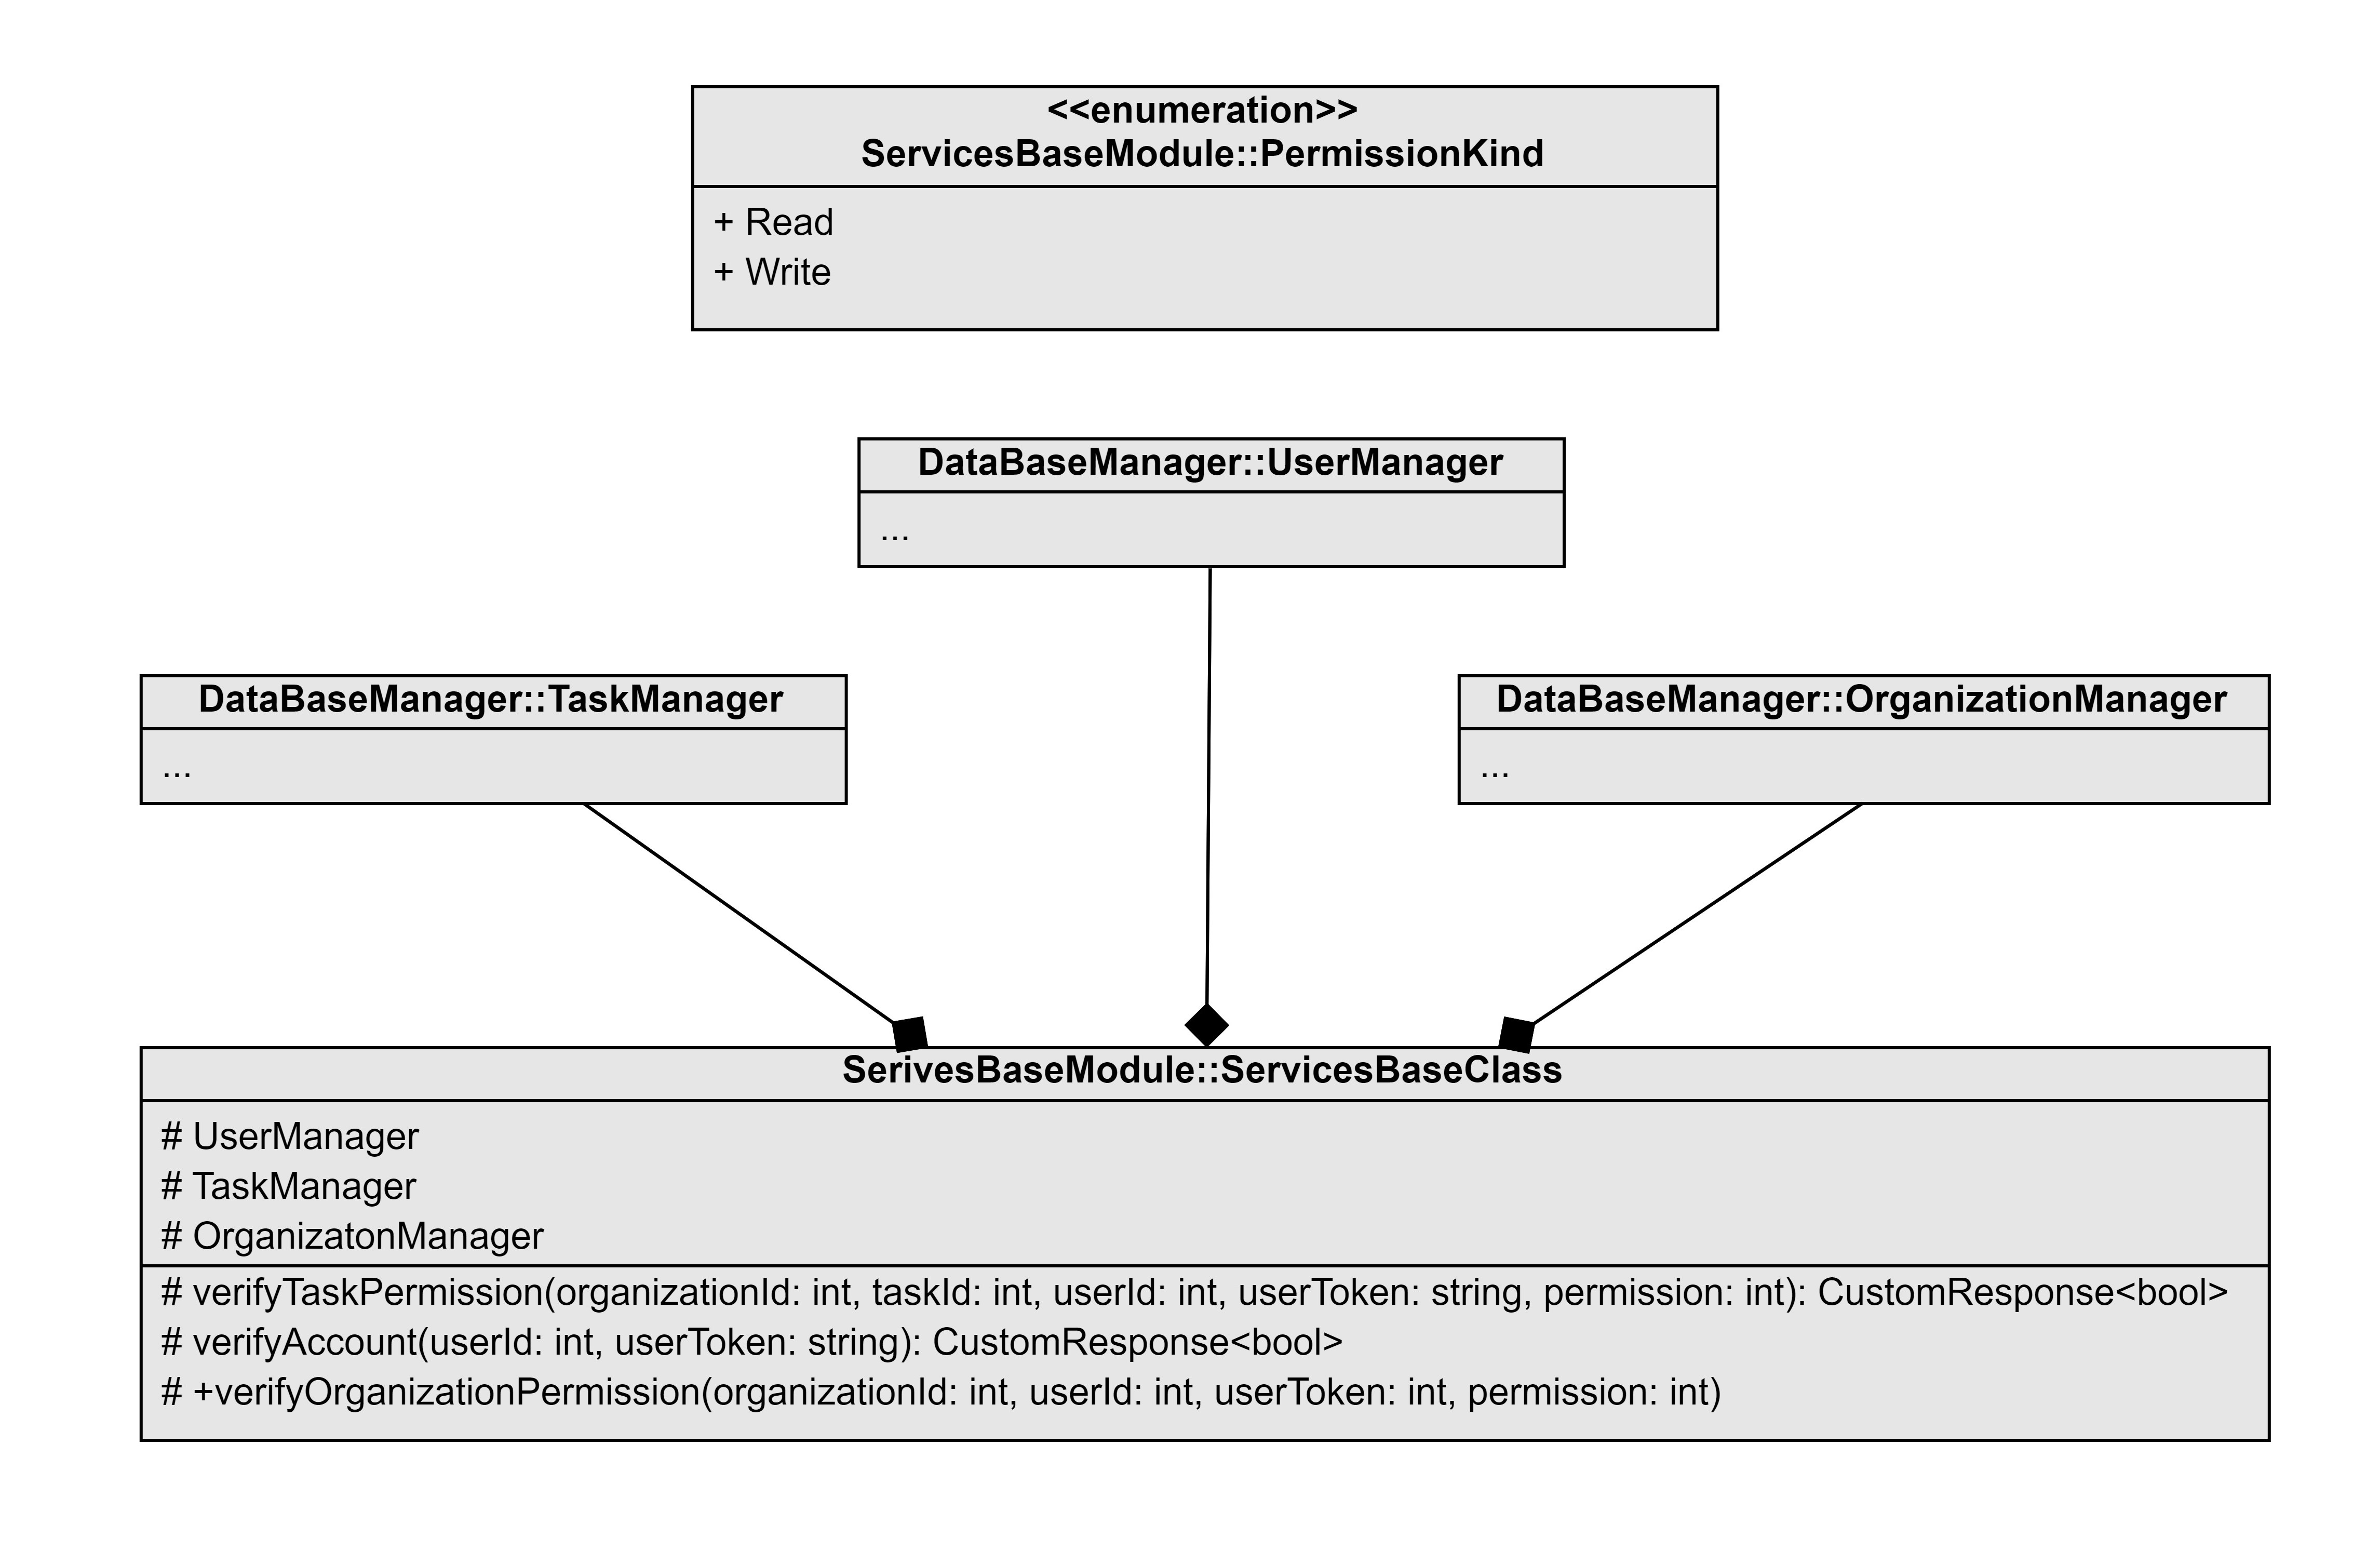
\includegraphics[width=\textwidth,height=\textheight,keepaspectratio]{images/class_diagram/services_base_.jpg}

\subsubsection{Description}

The Services Base Module is used to intercommunicate directly with the Data Base Manager and its classes as mentioned above (Task, User and Organization Manager).

An enum is necessary to rappresents the Read and Write permision attributes. The relates the 3 classes of the Data Base Manager mentioned above and provides the methods to verify the user, the permission of the task and the permission of the organization.

\subsection{Notification System}
\subsubsection{Diagram}

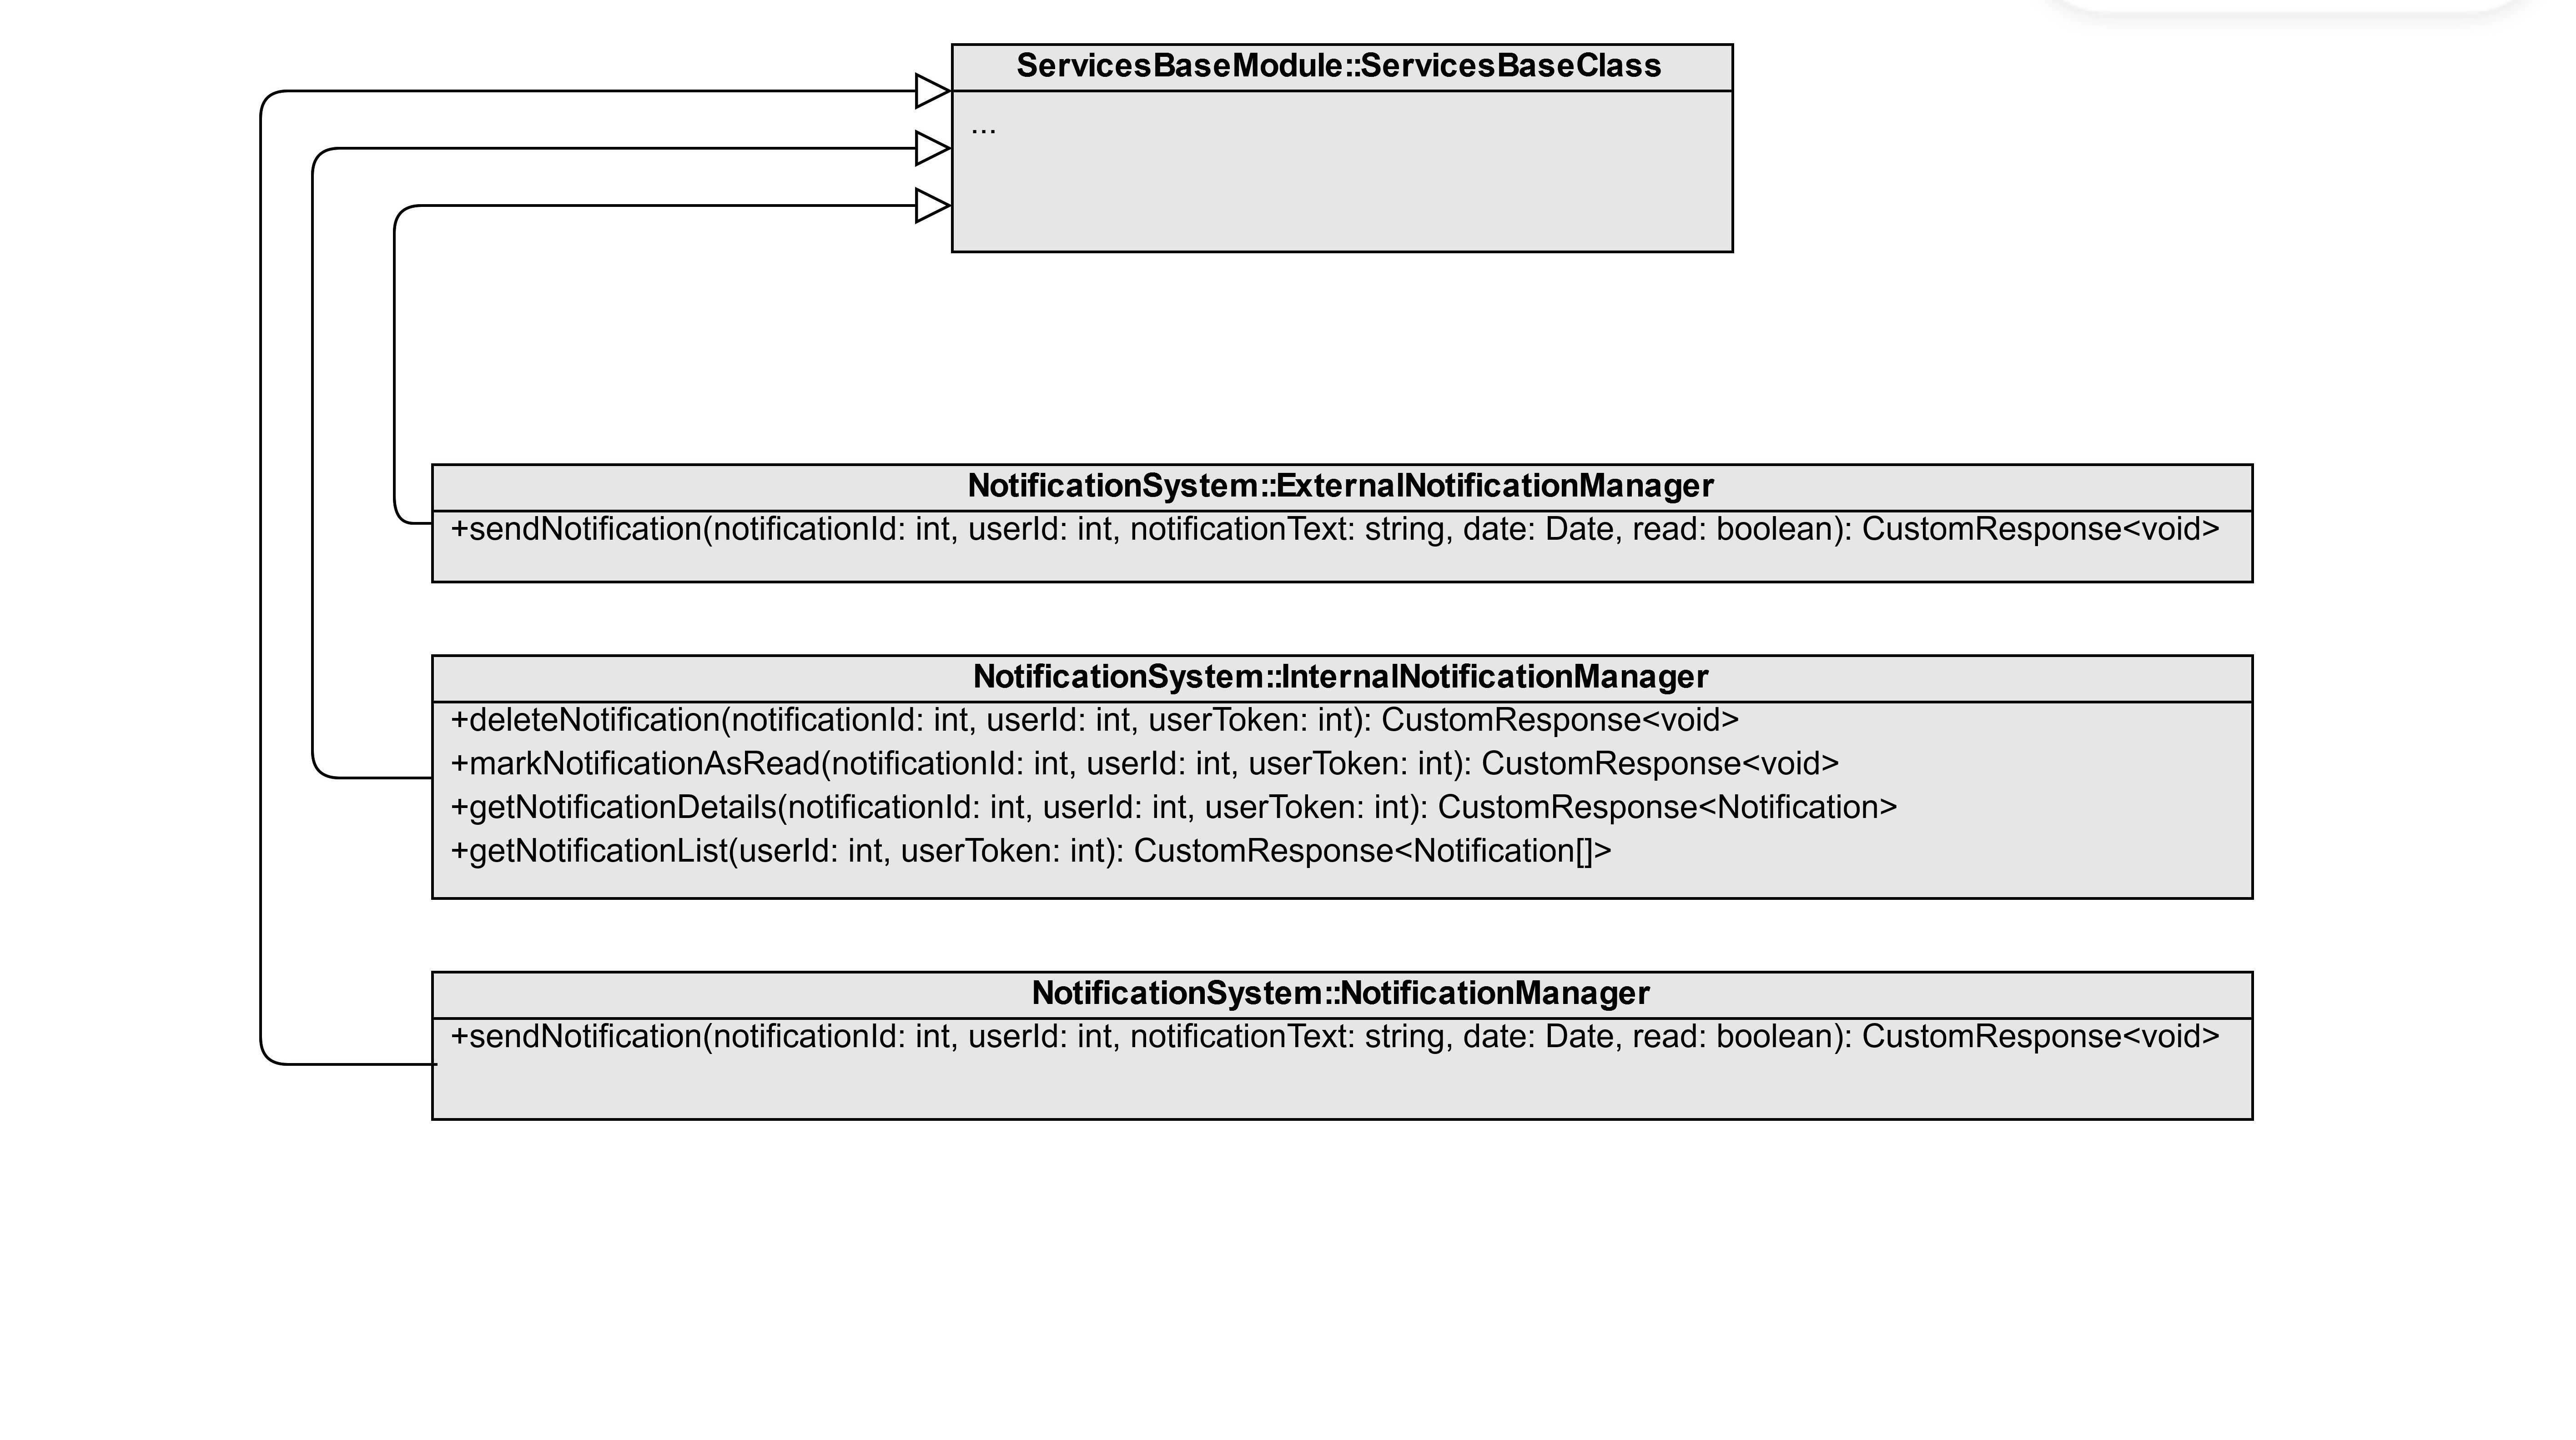
\includegraphics[width=\textwidth,height=\textheight,keepaspectratio]{images/class_diagram/notificationSystem.jpg}

\subsubsection{Description}

The notification system is used to send notifications to users, using both internal and external managers, and to view and handle existing notifications. Every notification is associated with a specific user, a date and a flag to see if it has been read by the user. The system is composed by:

\begin{itemize}

\item \textbf{External Notification Manager}

This class refers to the external notification system. It implements the possibility to send notifications using mails to a specific user. 

\item \textbf{Internal Notification Manager}

This class refers to the internal notification system, that works in-app. It is possible to delete sent notifications, to mark them as read or unread, to get details about one of them and to get the list of notifications associated to a specific user.

\item \textbf{Notification Manager}

This class refers to the generic notifications handler. The component acts as a switch, so it decides whether a notification should be sent via external or internal system.
\end{itemize}

\subsection{Task Manager} %gab
\subsubsection{Diagram}
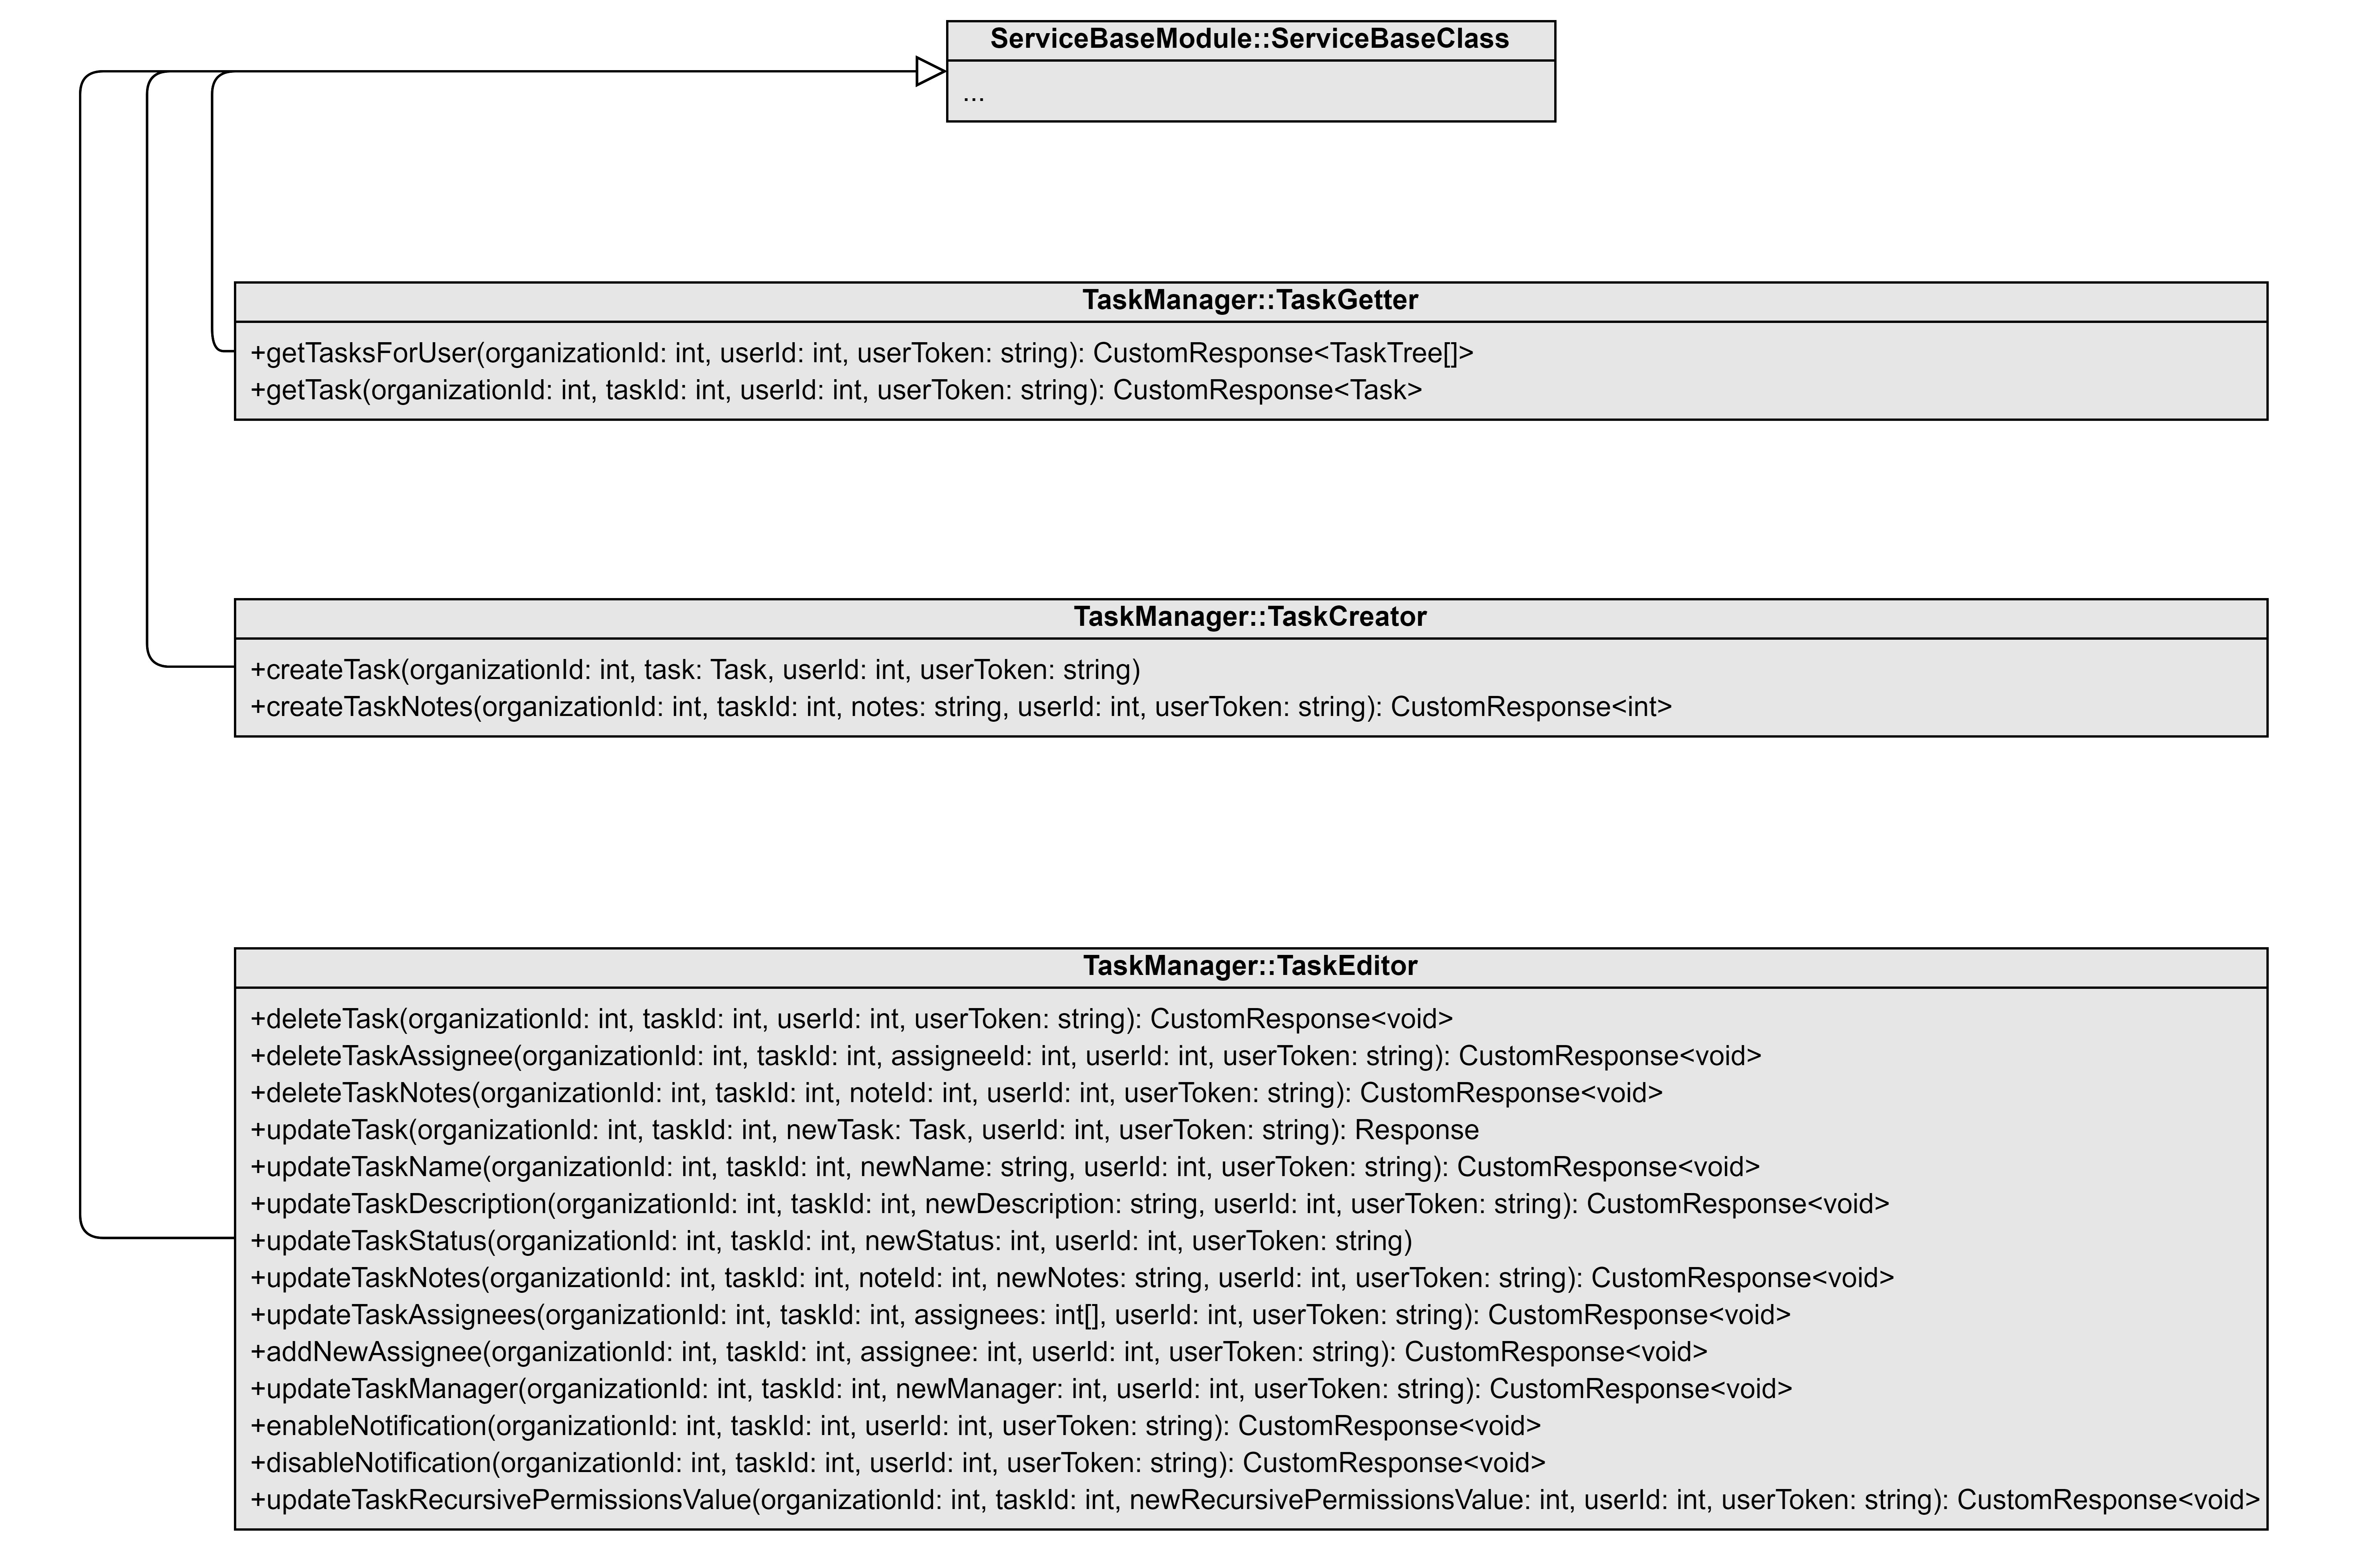
\includegraphics[width=\textwidth, height=\textheight, keepaspectratio]{images/class_diagram/task_manager.jpg}
\subsubsection{Description}
The Task Manager module allows users to interact with the tasks. Here is a list containing each class of this module:
\begin{itemize}
    \item \textbf{TaskGetter}
    This class returns any task requested by the user for his specific organization. It can either respond with the entire task tree or a specific one.
    \item \textbf{TaskCreator}
    This class allows users to create new tasks, or even add notes to already existing ones.
    \item \textbf{TaskEditor}
    This class include various methods for task modification. Some of the functionalities included are:
    \begin{itemize}
        \item Addition and removal of assignees in a specified task
        \item Update task name
        \item Edit or delete task notes
        \item Edit or delete specified Task
        \item Enable or disable notification for specified task
    \end{itemize}
\end{itemize}
\subsection{User Manager}

\subsubsection{Diagram}

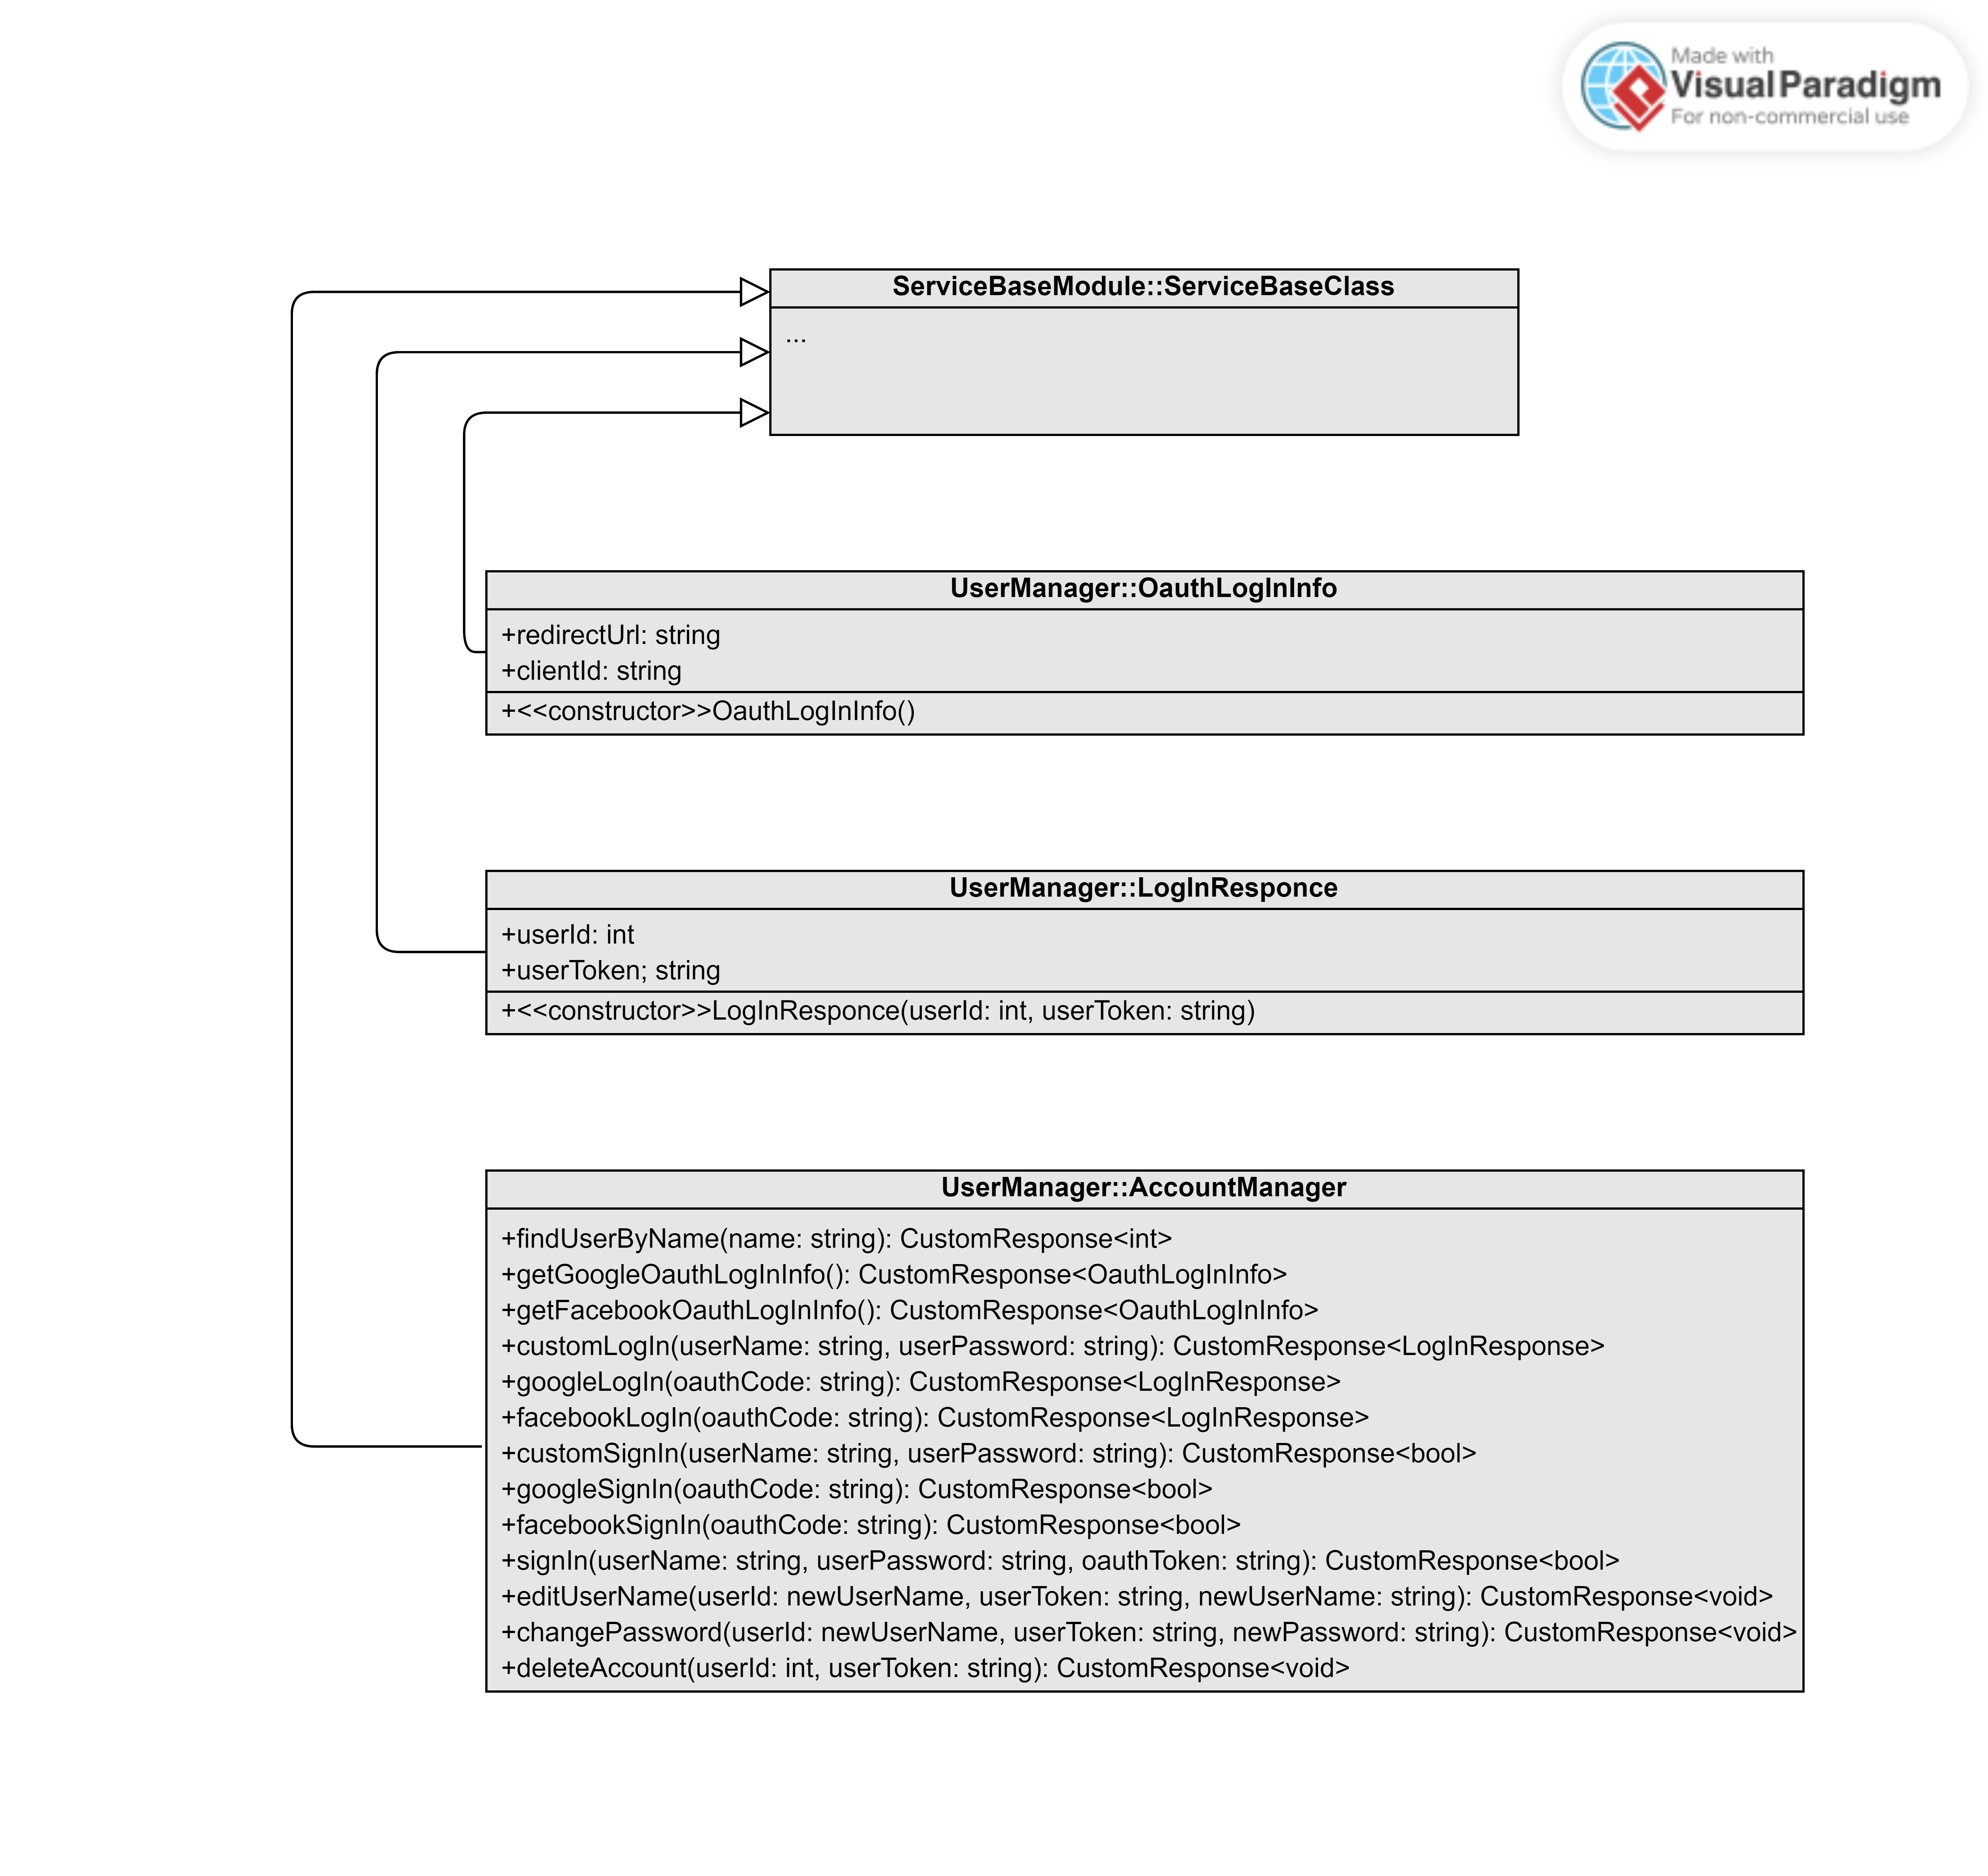
\includegraphics[width=\textwidth,height=\textheight,keepaspectratio]{images/class_diagram/user_manager.jpg}

\subsubsection{Description}

The User manager system is used to provide functionalities for the user's account management.

Once connected to the ServiceBaseClass discussed above, it provides the following classes:

\beging{itemize}
  \item \textbf{OauthLogInInfo: }
  
  A class which contains the link for the redirection and the clientId as a string.

  \item \textbf{LogInResponse: }
  
  A class containing the ID of the user and the string based on the response.

  \item \textbf{AccountManager: }

  A class which contains all the methods used to manage the accounts, such as the logins management via external APIs or the change of the password.

\subsection{Organization Manager}

\subsubsection{Diagram}
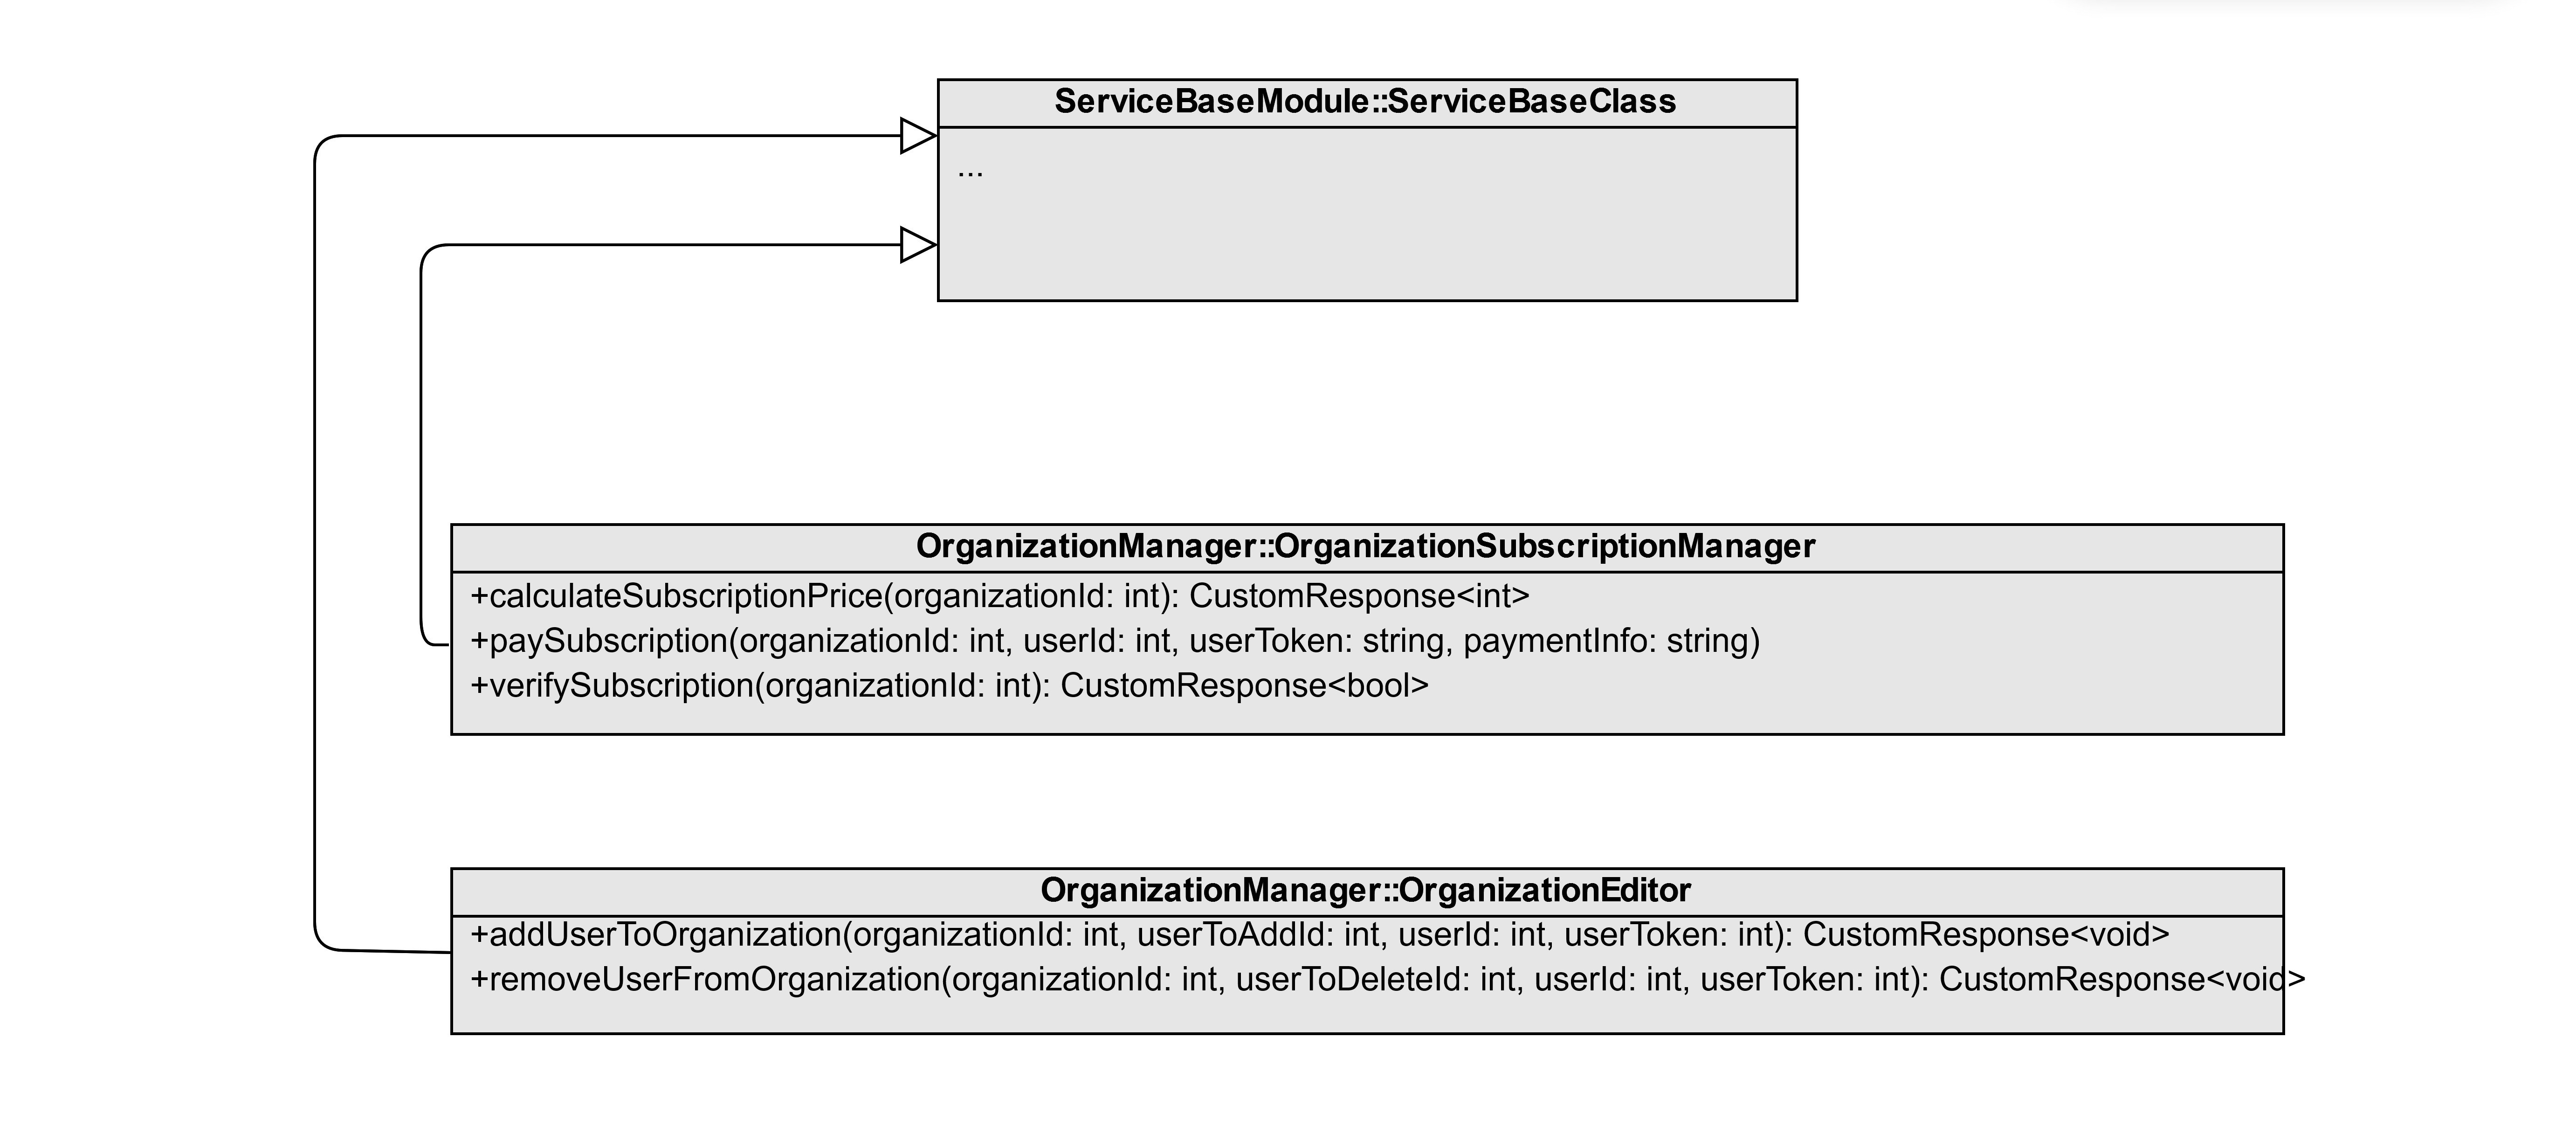
\includegraphics[width=\textwidth,height=\textheight,keepaspectratio]{images/class_diagram/OrganizationManager.jpg}
\subsubsection{Description}
The Organization Manager is used to Owners with functionalities that vary from subscription management to Organization management
\begin{itemize}
    \item \textbf{OrganizationSubscriptionManagement}
    This class handles the subscription side of the Organization. It contains methods for:
    \begin{itemize}
        \item subscription verification and payment
        \item calculation of total subscription fee
    \end{itemize}
    \item \textbf{OrganizationEditor}
    This class allows Owners to add and remove new members in the Organization

\end{itemize}
\subsection{Report Manager} % Luca non s

\subsubsection{Diagram}

\includegraphics[width=\textwidth,height=\textheight,keepaspectratio]{images/class_diagram/reportManager.jpg}

\subsubsection{Description}

The report manager is responsible for generating reports and managing report schedule. It is composed by:

\begin{itemize}

\item \textbf{Automatic Report Manager}
This class refers to the automatic report generation, implementing the possibility to generate the report. It is connected to external APIs that will use information available in the database to complete the process.

\item \textbf{Manual Report Manager}
This class refers to the manual report generation, so report that are realised manually by users on request.

\item \textbf{Report Manager}

This class refers to the generic report manager, that will decide if a report should be generated automatically or manually.

\item \textbf{Report Scheduler}

This class referes to the report scheduler management. It implements the possibility to schedule the sending of a report, get a list of the scheduled reports for a specific user, delete report requests scheluled for a specific user and execute report request that have been scheduled.

\end{itemize}

\end{document}
